% !TeX program = xelatex
% Figures are relative to this source.
% Figure text is calibrated to 8--9 pt at the includegraphics widths below.
\documentclass[a4paper,12pt]{article}
\usepackage{fontspec,xeCJK}
\usepackage{graphicx,amsmath,amssymb,array,tabularx,booktabs}
\usepackage{float,caption,titlesec,geometry,xcolor,listings,xurl}
\usepackage[hidelinks]{hyperref}
\usepackage{bookmark}
\usepackage[section]{placeins}
\IfFontExistsTF{Songti SC}{\setCJKmainfont[AutoFakeBold=2.5]{Songti SC}}{\setCJKmainfont{FandolSong-Regular}}
\IfFontExistsTF{Heiti SC}{\setCJKsansfont[AutoFakeBold=2.5]{Heiti SC}}{\setCJKsansfont{FandolHei-Regular}}
\IfFontExistsTF{Kaiti SC}{\setCJKmonofont{Kaiti SC}}{\setCJKmonofont{FandolKai-Regular}}
\IfFontExistsTF{Times New Roman}{\setmainfont{Times New Roman}}{\setmainfont{TeX Gyre Termes}}
\IfFontExistsTF{Menlo}{\setmonofont{Menlo}[Scale=0.85]}{\setmonofont{Latin Modern Mono}[Scale=0.85]}
\XeTeXlinebreaklocale "zh"
\XeTeXlinebreakskip=0pt plus 1pt minus 0.1pt
\newcommand{\xiaoyi}{\fontsize{24pt}{36pt}\selectfont}
\newcommand{\erhao}{\fontsize{22pt}{28pt}\selectfont}
\newcommand{\xiaoer}{\fontsize{18pt}{24pt}\selectfont}
\newcommand{\xiaosan}{\fontsize{15pt}{22pt}\selectfont}
\newcommand{\sihao}{\fontsize{14pt}{21pt}\selectfont}
\newcommand{\xiaosi}{\fontsize{12pt}{18pt}\selectfont}
\geometry{left=3.18cm,right=3.18cm,top=2.54cm,bottom=2.54cm}
\titleformat{\section}{\sffamily\sihao\bfseries}{\thesection}{1em}{}
\titleformat{\subsection}{\sffamily\xiaosi\bfseries}{\thesubsection}{1em}{}
\titlespacing*{\section}{0pt}{0.9em}{0.45em}
\titlespacing*{\subsection}{0pt}{0.7em}{0.3em}
\setlength{\parindent}{2em}
\setlength{\parskip}{0.25em}
\setlength{\emergencystretch}{2em}
\renewcommand{\arraystretch}{1.18}
\captionsetup{font=small,labelfont=bf,labelsep=colon}
\renewcommand{\figurename}{图}
\renewcommand{\tablename}{表}
\renewcommand{\refname}{参考文献}
\newcolumntype{Y}{>{\raggedright\arraybackslash}X}
\definecolor{codebg}{RGB}{244,246,248}
\lstset{backgroundcolor=\color{codebg},basicstyle=\ttfamily\footnotesize,
 breaklines=true,columns=fullflexible,keepspaces=true,frame=single,
 rulecolor=\color{codebg},showstringspaces=false,aboveskip=0.6em,belowskip=0.6em}
\urlstyle{tt}
\newcommand{\ReportTitle}{环加成反应的机理研究}
\newcommand{\kcalmol}{\mathrm{kcal\,mol^{-1}}}
\hypersetup{pdftitle={环加成反应的机理研究},pdfauthor={叶青杨}}

\begin{document}
\begin{titlepage}
\centering
\vspace*{1cm}
{\xiaoyi\bfseries 浙江大学量子化学实验\par}
\vspace{1cm}
{\sffamily\xiaoer \ReportTitle\par}
\vspace{0.7cm}
{\sffamily\erhao\bfseries 实\\[0.32cm]验\\[0.32cm]报\\[0.32cm]告\par}
\vfill
{\sihao 参加学生：叶青杨\par}
\vspace{1cm}
{\xiaoer\bfseries 浙江大学化学实验教学中心\par}
\vspace{0.5cm}
{\xiaoer\bfseries 2026年10月15日\par}
\end{titlepage}
\setcounter{page}{1}
\begin{center}
{\sffamily\xiaosan\bfseries \ReportTitle\par}
\vspace{0.4em}
{\xiaosi 叶青杨\par}
\end{center}
\xiaosi

\section{实验目的}
以 1,3-丁二烯与乙烯生成环己烯的 Diels--Alder 反应为对象，学习限制性优化、过渡态搜索与频率分析，利用内禀反应坐标（IRC）确认反应通道；比较各驻点的 Gibbs 自由能，并通过前线轨道相位解释协同成键特征\cite{course}。进一步比较环己烯的两个局部稳定构象，并以顺丁烯二酸酐为亲双烯体，比较两种环加成反应的势垒与成键路径。

\section{实验原理与计算方法}
\subsection{驻点、频率与反应路径}
在 Born--Oppenheimer 势能面上，驻点满足 $\nabla E=0$。质量加权 Hessian 的本征值决定振动频率的平方；扣除整体平移和转动后，局部极小值的 $3N-6$ 个振动本征值均为正，一阶鞍点恰有一个负本征值。与该负本征值对应的虚频模式给出势能下降方向。IRC 从过渡态沿质量加权坐标中的最陡下降方向追踪两侧势能面，通过端点优化确定所连接的极小值。

本实验的共同碳编号为：丁二烯 C1--C2--C3--C4，乙烯 C5--C6；形成的新键为 C1--C5 和 C4--C6，环己烯中保留 C2=C3 双键。

\subsection{电子结构计算}
主要计算采用 Gaussian 16 的 B3LYP-D3(BJ)/def2-SVP 方法，在气相、中性单重态条件下进行。D3(BJ) 为带 Becke--Johnson 阻尼的色散修正。Gaussian 各步骤统一采用 \texttt{SCF=(Tight,XQC)}、\texttt{Int=UltraFine} 和 \texttt{NoSymm}。普通极小值的主要输入为
\begin{lstlisting}
#p B3LYP/Def2SVP EmpiricalDispersion=GD3BJ
   SCF=(Tight,XQC) Int=UltraFine NoSymm
   Opt=(CalcFC,Tight,MaxCycles=200) Freq
\end{lstlisting}
独立丁二烯的初始中央单键扭角设为 $30^\circ$，随后自由优化；环加成初猜则采用平面 s-cis 丁二烯，使乙烯靠近两端，并将两条形成键均设为 $2.27\ \mathrm{\AA}$。

先冻结两条形成键距离，优化其余自由度：
\begin{lstlisting}
Opt=(ModRedundant,CalcFC,Tight,MaxCycles=200)

B 1 5 F
B 4 6 F
\end{lstlisting}
以所得结构为初猜，删除冻结坐标，进行无约束过渡态优化和频率分析：
\begin{lstlisting}
Opt=(TS,CalcFC,NoEigenTest,Tight,MaxCycles=200) Freq
\end{lstlisting}
限制性优化所得结构用于过渡态搜索，热力学量取自最终无约束驻点。通过收敛梯度、唯一虚频及 IRC 连接关系确定过渡态。

另以 ASE/ORCA 6.1.1 进行距离引导的 CI-NEB 复核。电子结构模型为 B3LYP-D3(BJ)/def2-SVP，ORCA 采用 \texttt{B3LYP/G}、\texttt{NoRI NoCOSX VeryTightSCF DEFGRID3}；其中 \texttt{B3LYP/G} 对应 Gaussian 的泛函定义，积分网格采用 ORCA 的 DEFGRID3\cite{orca-dft}。弱结合复合物与环己烯 B 作为固定端点，共 17 个图像；以约 $2.27\ \mathrm{\AA}$ 的成键距离引导势垒附近的初猜加密，正式 NEB 中解除内部图像的全部几何约束。直接在最终爬山图像上，用解析梯度的中心差分（步长 $0.005\ \mathrm{bohr}$）计算独立数值 Hessian\cite{orca-freq}。

构象转化计算从分别优化并经独立数值频率验证的 A、B 出发，仅用端点插值和 IDPP 构建 17 图像初猜。普通 NEB 与 CI-NEB 的整带最大有效力判据分别为 $0.05$ 与 $0.01\ \mathrm{eV\,\AA^{-1}}$；爬山图像随后进行无约束 OptTS 精修及独立数值 Hessian 计算。NEB 沿路径比较电子能，驻点自由能另由频率热校正得到。

\subsection{IRC 与热化学处理}
环加成 IRC 从最终过渡态几何及频率计算的 Hessian 出发，分别追踪两个方向，采用 RCFC/HPC、Tight 收敛及定期 Hessian 更新。初始名义步长为 $0.10\ \mathrm{bohr}$，反应物侧近端点段采用 $0.05\ \mathrm{bohr}$。检查每个接受点的能量、反应坐标与成键距离，并对两端结构分别优化、计算频率。

热化学量采用 $298.15\ \mathrm{K}$、$1\ \mathrm{atm}$ 下的理想气体刚性转子--谐振子（RRHO）近似，频率不缩放。$G_{\rm out}$ 直接取最终频率输出的 \texttt{Sum of electronic and thermal Free Energies}，其中已含零点能与热校正\cite{thermo}。外转动对称数按保持原子种类和连接关系的正旋转确定；若其与输出采用的值不同，则
\begin{equation}
G=G_{\rm out}+RT\ln\frac{\sigma}{\sigma_{\rm out}}.
\label{eq:sigma}
\end{equation}
乙烯的 $\sigma=4$，丁二烯与环己烯 A 的 $\sigma=2$，其余驻点为 1。丁二烯与 A 的输出采用 $\sigma_{\rm out}=1$，故各加入 $RT\ln2=0.41\ \kcalmol$；其余不变。镜面反射不计入外转动对称数。

以本次优化的近 s-cis 扭曲丁二烯与乙烯两个分离反应物为参考，定义
\begin{align}
\Delta G^{\ddagger}&=G(\mathrm{TS})-[G(\text{丁二烯})+G(\text{乙烯})],\\
\Delta_{\mathrm r}G&=G(\text{环己烯})-[G(\text{丁二烯})+G(\text{乙烯})].
\end{align}
每种物质采用单一优化构象的配分函数。Hartree 与能量单位的换算采用 $1\ E_{\rm h}=627.5095\ \kcalmol$。结果通常显示至能量小数点后两位、键长后三位及频率后一位；微小差值单独保留必要有效数字，能量差均由未舍入数据计算。

\section{结果与分析}
\subsection{优化结构与过渡态的确认}
乙烯、丁二烯及环己烯 A 均得到无虚频的局部极小值（图~\ref{fig:structures}）。丁二烯的 C1--C2--C3--C4 二面角为 $26.90^\circ$，属于近 s-cis 扭曲构象，而不是平面 s-cis 结构。

\begin{figure}[htbp]
\centering
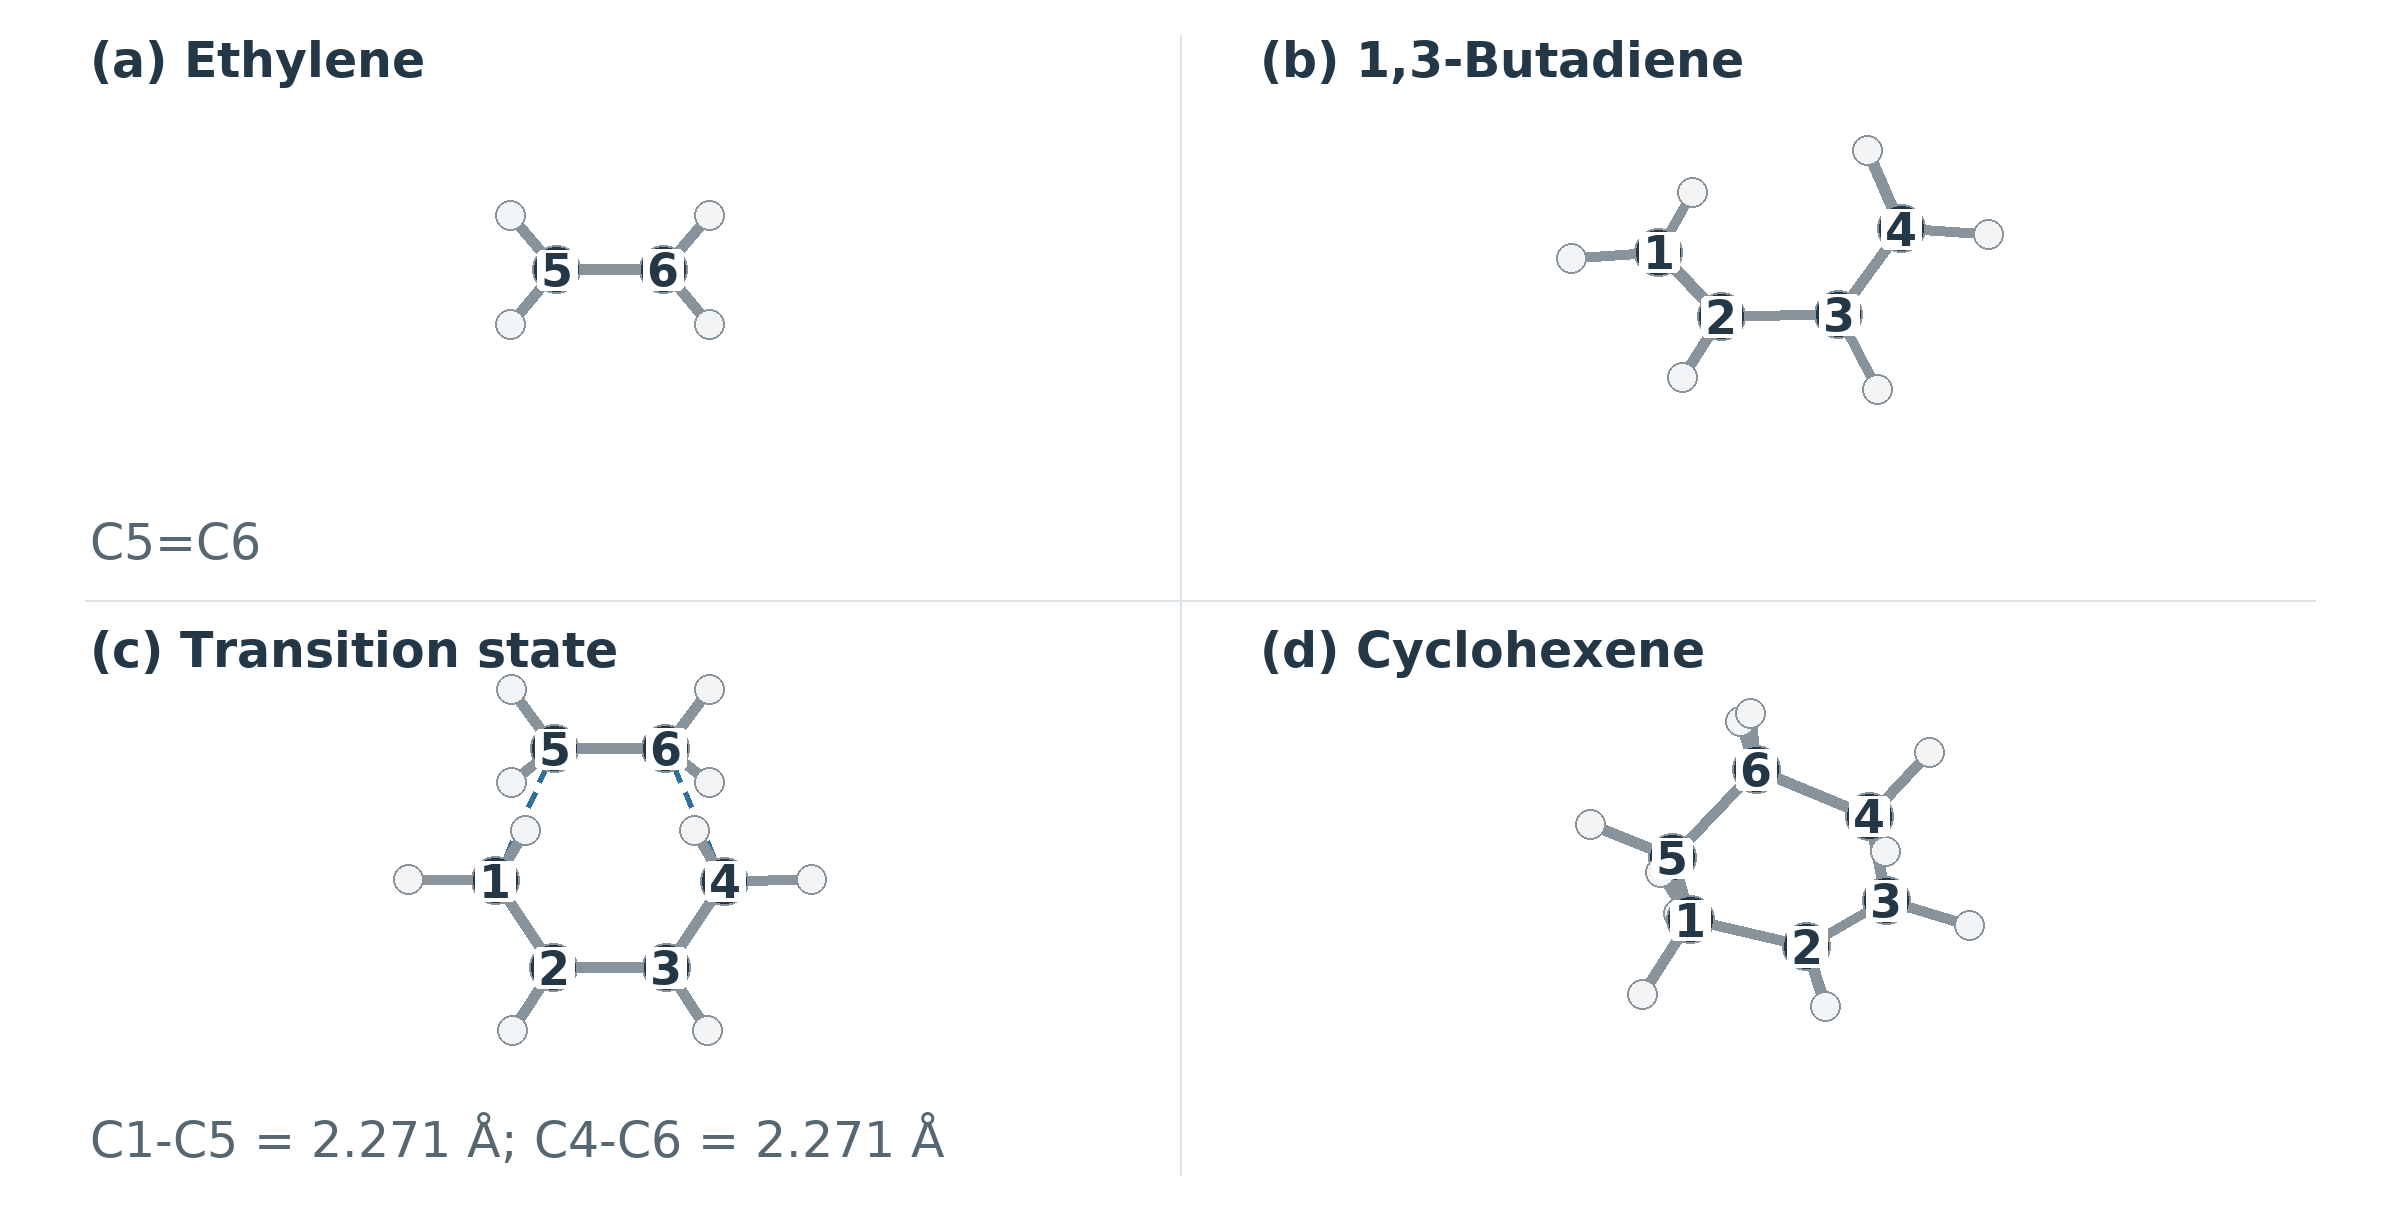
\includegraphics[width=\linewidth]{figures/optimized-structures.png}
\caption{独立反应物、环加成过渡态及环己烯 A 的优化结构，采用统一分子尺度。碳编号为丁二烯 C1--C4、乙烯 C5--C6，虚线标出两条形成键。丁二烯二面角为 $26.90^\circ$；各结构的振动数及虚频见表~\ref{tab:frequency}。图中环己烯为独立优化构象 A；IRC 直接连接的 B 见图~\ref{fig:irc-structures}。}
\label{fig:structures}
\end{figure}

\begin{table}[htbp]
\centering\small
\caption{各驻点的振动分析。频率单位为 $\mathrm{cm^{-1}}$。}
\label{tab:frequency}
\begin{tabular}{lrrr}
\toprule
体系 & 模式总数 & 虚频数 & 最低频率\\
\midrule
乙烯 & 12 & 0 & 822.9\\
近 s-cis 丁二烯 & 24 & 0 & 138.1\\
反应物复合物 & 42 & 0 & 29.6\\
环加成 TS & 42 & 1 & $517.2i$\\
环己烯 B & 42 & 0 & 45.5\\
环己烯 A & 42 & 0 & 170.1\\
\bottomrule
\end{tabular}
\end{table}

环加成过渡态的 42 个振动模式中恰有一个虚频 $517.2i\ \mathrm{cm^{-1}}$。其位移使 C1--C5 与 C4--C6 同时缩短或伸长（图~\ref{fig:mode}）。两条形成键分别为 $2.271$ 和 $2.271\ \mathrm{\AA}$，相差仅约 $2\times10^{-5}\ \mathrm{\AA}$，显示该过渡态具有近同步的双端成键特征。

\begin{figure}[htbp]
\centering
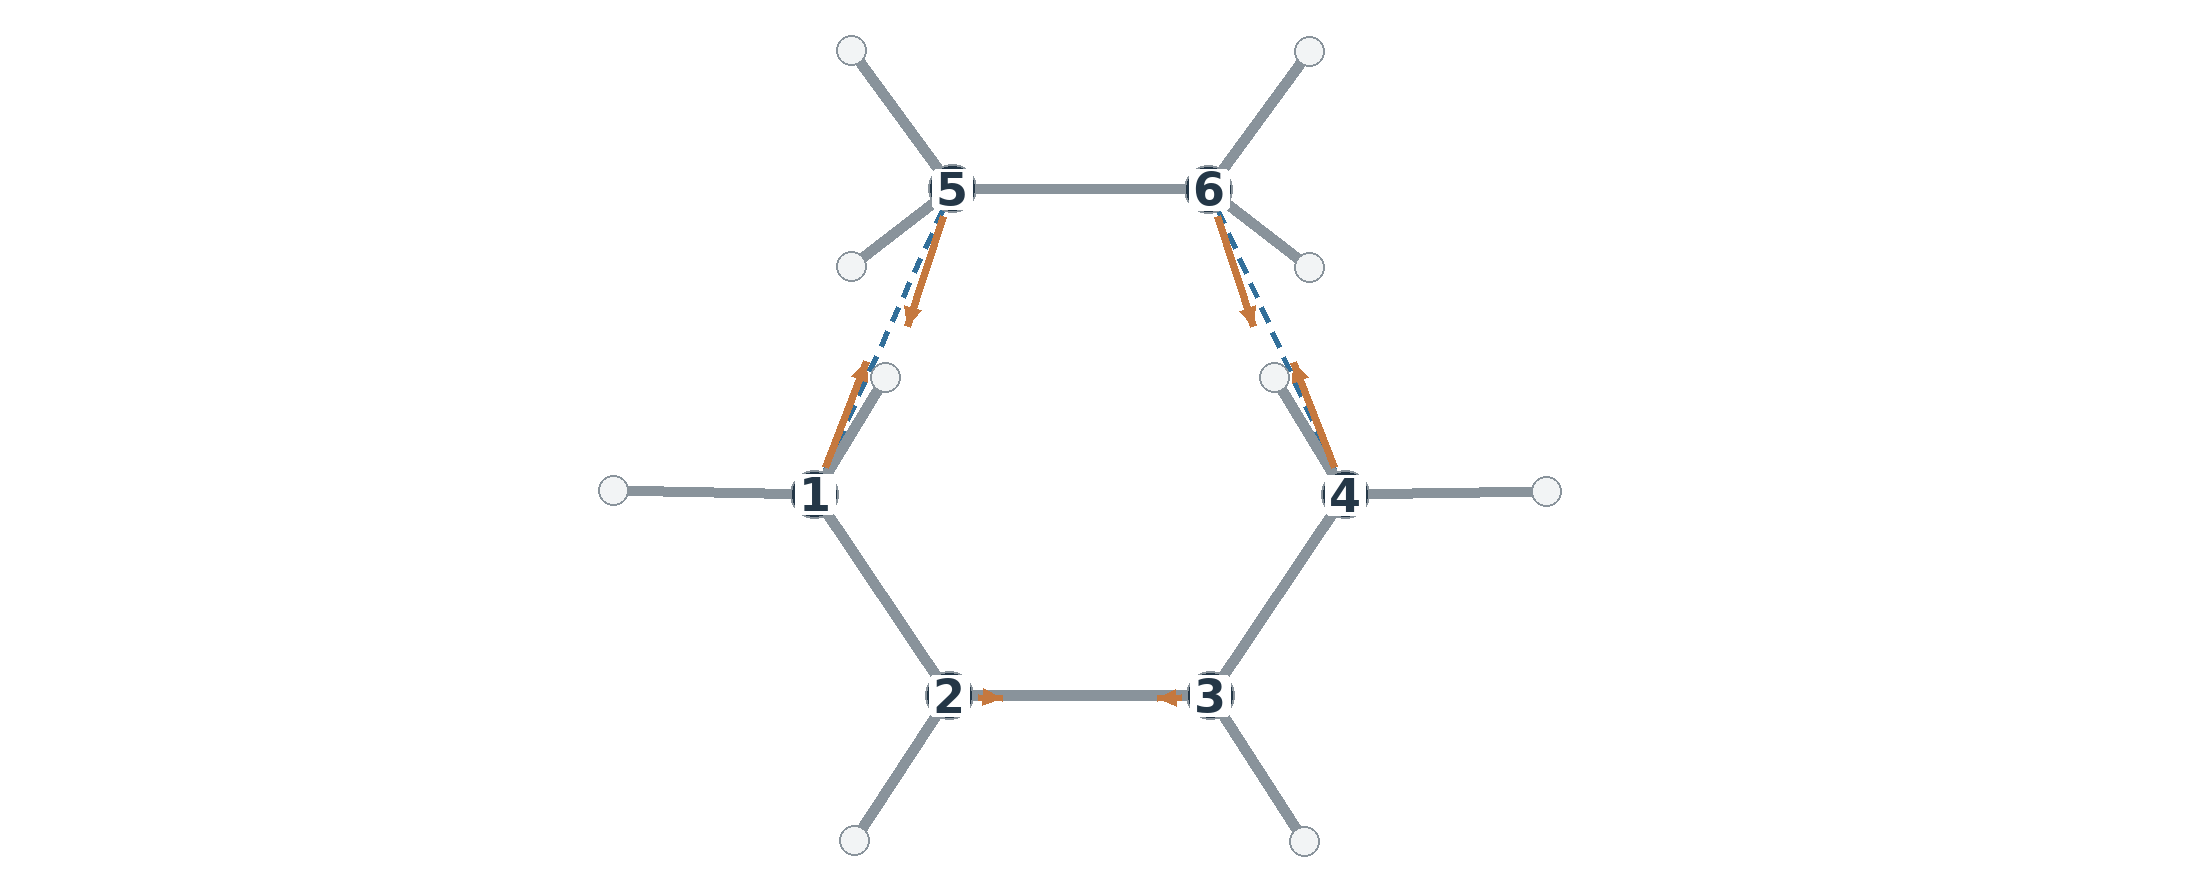
\includegraphics[width=0.91\linewidth]{figures/ts-imaginary-mode.png}
\caption{环加成过渡态的唯一虚频模式，频率为 $517.2i\ \mathrm{cm^{-1}}$。箭头为放大的正常模式位移，所示方向对应两条新键协同形成，反向位移对应协同断裂；该位移不是 IRC 轨迹。}
\label{fig:mode}
\end{figure}

\subsection{IRC 路径与端点结构}
双向路径共包含 54 个接受点：反应物侧 34 点、产物侧 20 点。以 TS 的电子能为零点，沿两侧路径能量均下降（图~\ref{fig:irc}）；两条新键距离随路径近乎同步变化。此处横坐标为质量加权反应坐标，图中将反应物侧定义为负、产物侧定义为正。

\begin{figure}[htbp]
\centering
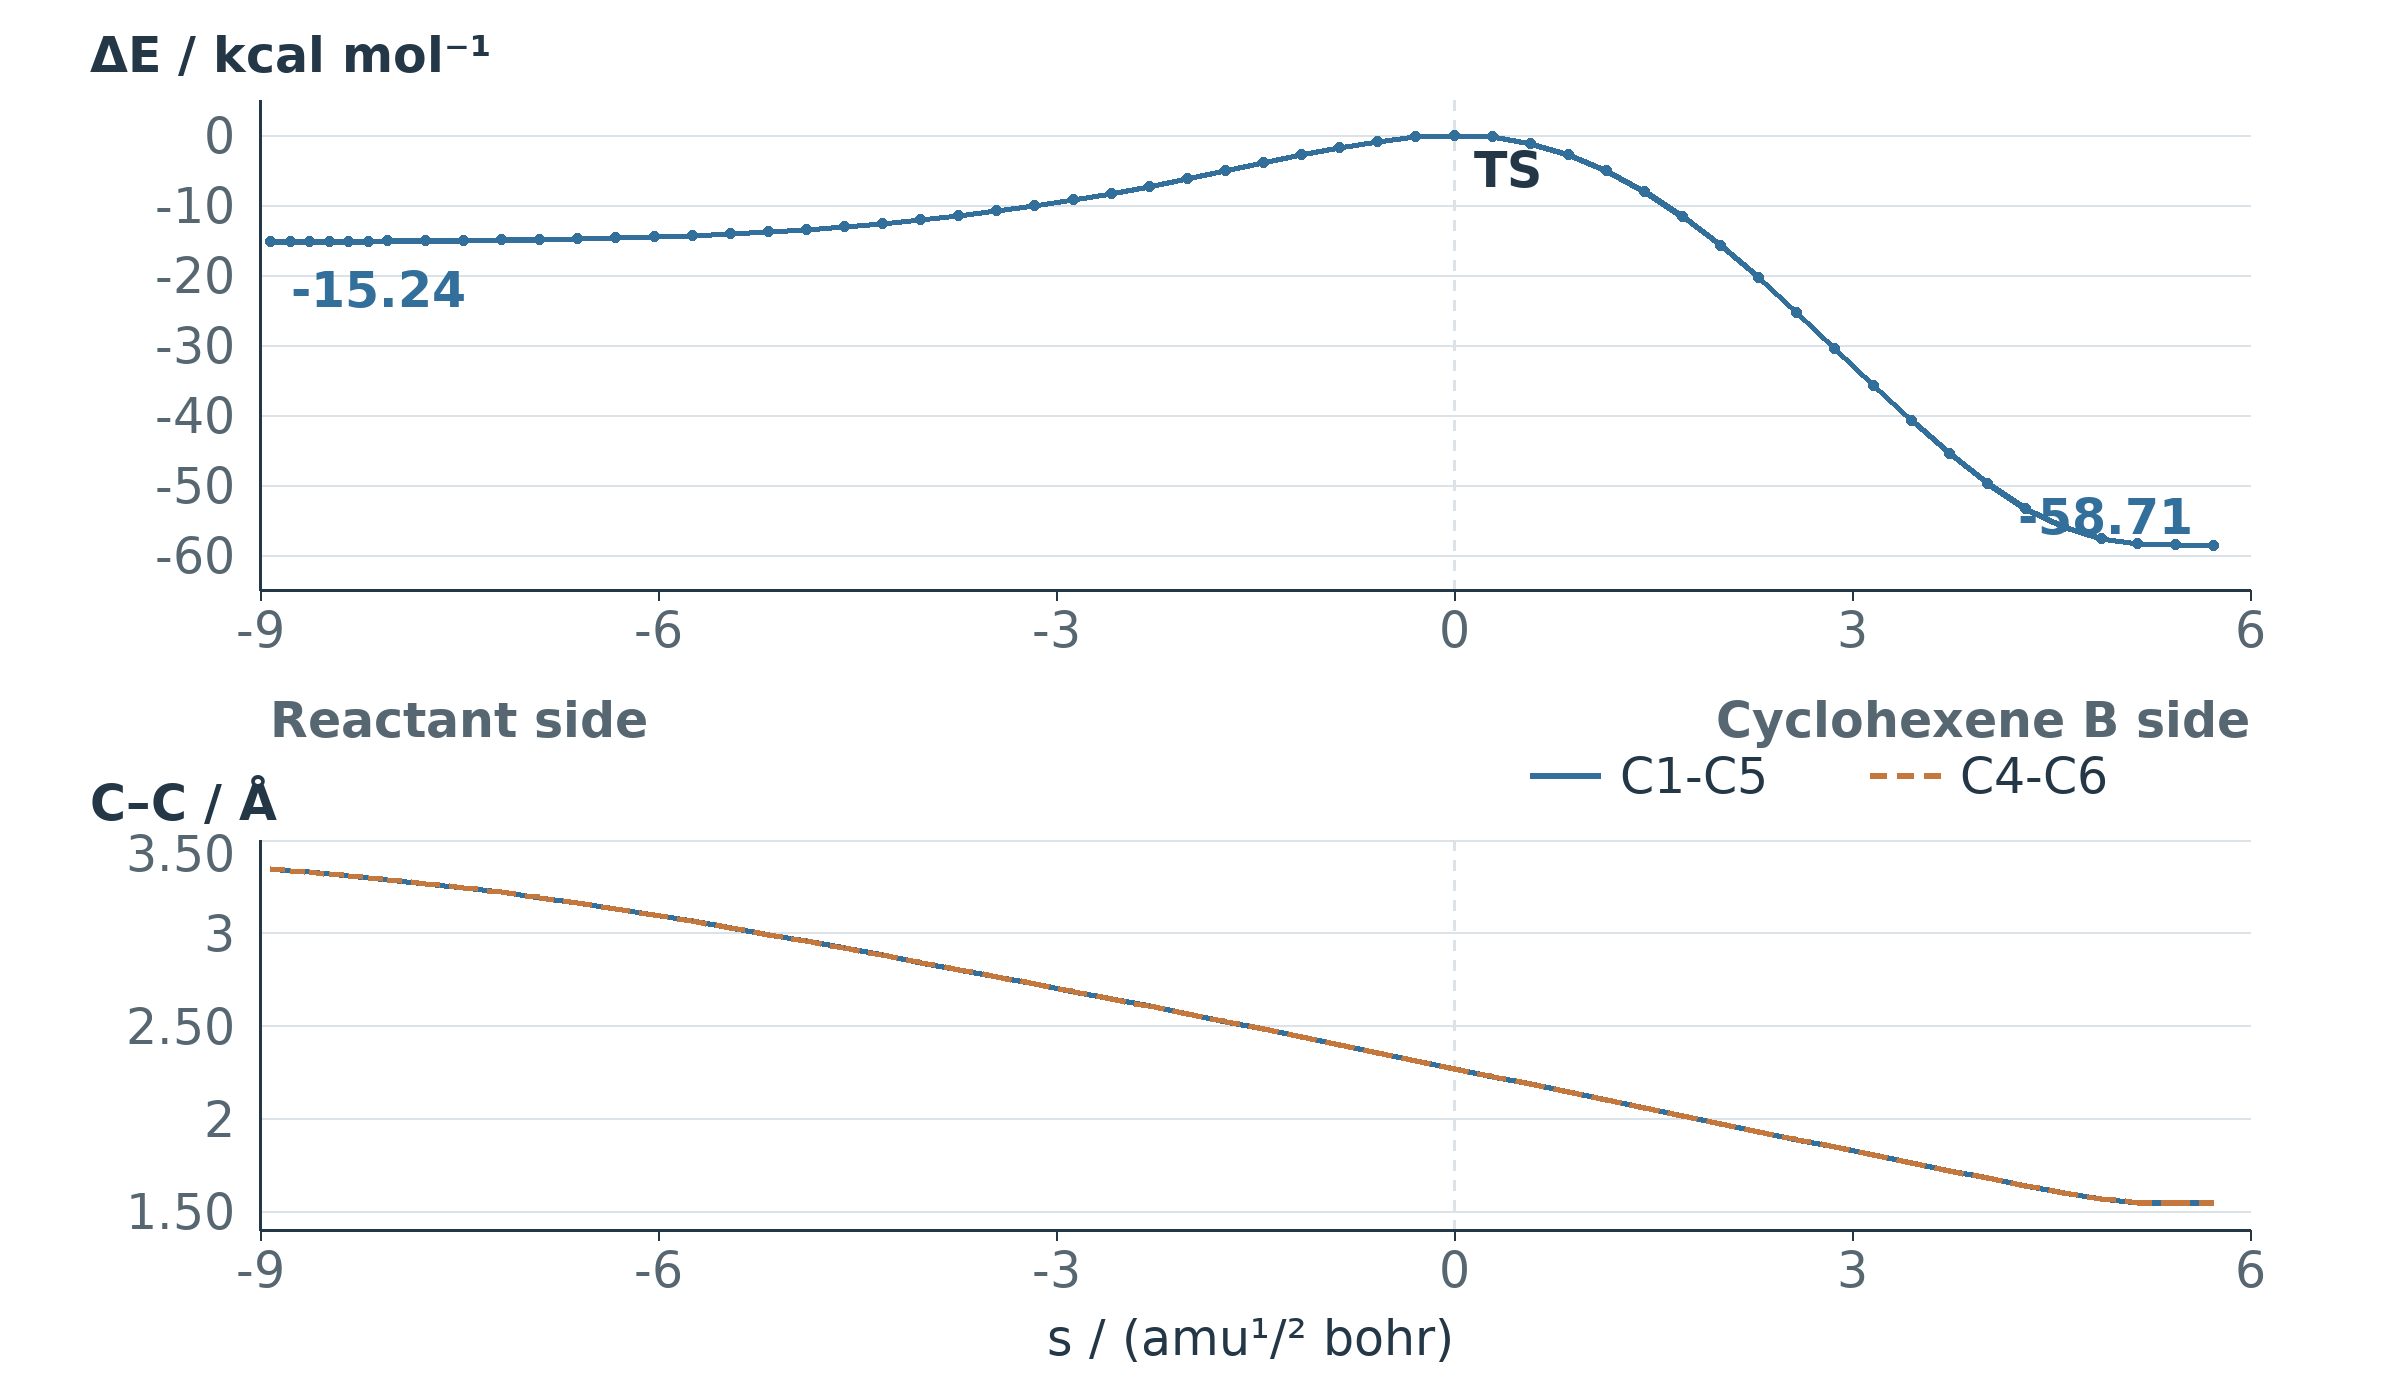
\includegraphics[width=\linewidth]{figures/irc-full-profile.png}
\caption{环加成 IRC 的电子势能和两条成键距离，共含 54 个收敛路径点及 TS。电子能以 TS 为零点；质量加权坐标 $s$ 的负、正方向分别为反应物侧和产物侧。曲线连接逐点计算结果，两端另行优化核验。}
\label{fig:irc}
\end{figure}
\begin{figure}[htbp]
\centering
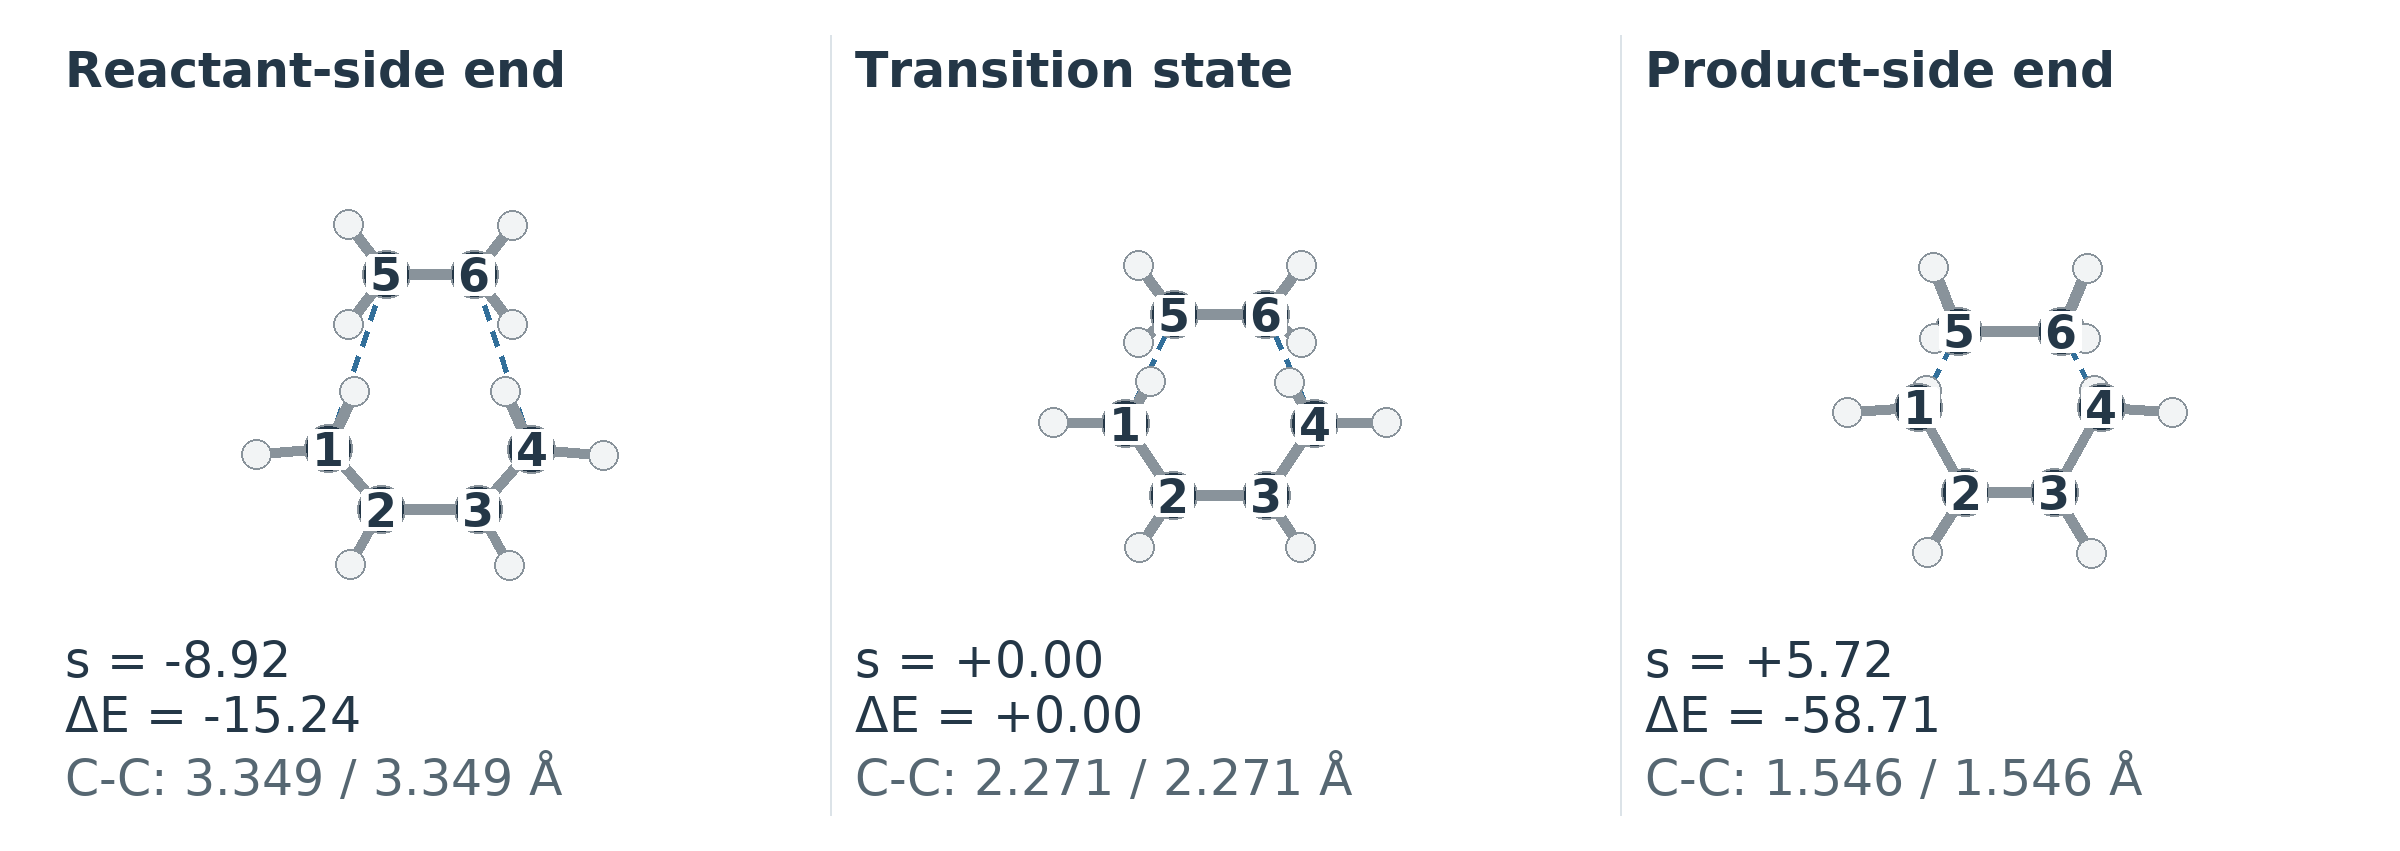
\includegraphics[width=\linewidth]{figures/irc-full-structures.png}
\caption{IRC 两端与 TS 的代表结构，采用统一尺度和碳编号。电子能以 TS 为零点，$\Delta E$ 的单位为 $\kcalmol$，$s$ 的单位为 $\mathrm{amu^{1/2}\,bohr}$，虚线标出 C1--C5 和 C4--C6。左右结构为路径末点，随后进行无约束优化及频率分析。}
\label{fig:irc-structures}
\end{figure}

反应物侧端点经优化得到丁二烯--乙烯弱结合复合物，42 个模式均为实频；$\mathrm{C1\cdots C5}$ 与 $\mathrm{C4\cdots C6}$ 距离为 $3.626$ 和 $3.657\ \mathrm{\AA}$，未形成新的共价键。碎片内部键长与独立反应物相比，最大差异分别为 $0.00065$ 和 $0.00125\ \mathrm{\AA}$。产物侧端点则得到环己烯 B，同样具有 42 个实频。其两条新键均为 $1.546\ \mathrm{\AA}$，C2=C3 为 $1.340\ \mathrm{\AA}$。因此，该过渡态连接反应物复合物与环己烯 B。

\begin{table}[htbp]
\centering\small
\caption{环加成 TS 与两个环己烯构象的主要碳--碳距离（$\mathrm{\AA}$）。}
\label{tab:bonds}
\begin{tabular}{lrrr}
\toprule
原子对 & TS & B & A\\
\midrule
C1--C2 & 1.383 & 1.506 & 1.507\\
C2--C3 & 1.409 & 1.340 & 1.340\\
C3--C4 & 1.383 & 1.506 & 1.507\\
C5--C6 & 1.386 & 1.552 & 1.532\\
C1--C5 & 2.271 & 1.546 & 1.534\\
C4--C6 & 2.271 & 1.546 & 1.534\\
\bottomrule
\end{tabular}
\end{table}
表~\ref{tab:bonds} 表明，反应过程中两条新 $\sigma$ 键形成，原丁二烯中央 C2--C3 键缩短为双键，而 C1--C2、C3--C4 与乙烯 C5--C6 均转为单键。唯一虚频、双端同步的距离变化及端点连接关系共同支持本通道的协同环加成机理。

\subsection{NEB、CI-NEB 与原 TS、IRC 的能垒比较}
普通 NEB 用离散图像逼近反应路径；CI-NEB 去除爬山图像的弹簧力，并反转沿路径方向的真实力分量，使该图像趋近鞍点\cite{ase-neb}。本节比较同一条 17 图像路径的普通 NEB 与 CI-NEB 末态，峰值均取最高图像的电子能。Gaussian IRC 以原优化 TS 为起点，沿两侧下降至反应物和产物区域\cite{orca-irc}。

两程序分别以同一弱结合复合物几何在本程序中的电子能为零点。表~\ref{tab:path-barriers} 中 CI-NEB 与 Gaussian 的电子能垒相差 $-0.0026\ \kcalmol$。在原 Gaussian TS 几何上以 ORCA 求能，得到复合物参照的高度 $15.74\ \kcalmol$，与 CI-NEB 峰顶仅差 $0.00012\ \kcalmol$，两种方法给出的电子势垒高度一致。

\begin{table}[htbp]
\centering\small
\caption{以各自程序的弱结合复合物为零点的电子势垒高度。}
\label{tab:path-barriers}
\begin{tabular}{lrp{6.3cm}}
\toprule
结果 & $\Delta E^\ddagger$ / $\kcalmol$ & 含义\\
\midrule
ORCA 普通 NEB & 15.74 & 最高离散图像\\
ORCA CI-NEB & 15.74 & 经独立数值频率分析的爬山图像\\
Gaussian 优化 TS & 15.74 & 原无约束优化得到的一阶鞍点\\
Gaussian IRC 的 TS 点 & 15.74 & 原优化 TS，双向 IRC 的共同起点\\
\bottomrule
\end{tabular}
\end{table}

普通 NEB 整带最大有效力为 $0.0413\ \mathrm{eV\,\AA^{-1}}$，达到 $0.05\ \mathrm{eV\,\AA^{-1}}$ 标准。峰顶真实最大原子力为 $0.0219\ \mathrm{eV\,\AA^{-1}}$，两条成键距离为 $2.267/2.267\ \mathrm{\AA}$。CI-NEB 将峰值能量提高了 $0.0021\ \kcalmol$，同时大幅降低峰顶残余力，使结构更接近驻点。

图~\ref{fig:path-comparison} 用两条成键距离的平均值 $q=[r(\mathrm{C1-C5})+r(\mathrm{C4-C6})]/2$ 对照三条路径，并按原始点序连线。三者呈现相同的总体成键趋势，峰顶接近，差别主要集中在反应物侧。CI-NEB 在这一侧的 $q$ 先增后减，反映了分子接近过程中的构型调整。NEB 的笛卡尔路径和 Gaussian 的质量加权 IRC 采用不同的路径度量，离散采样及其余自由度的变化也会影响投影曲线。

原 IRC 的反应物侧、产物侧最后一点分别比进一步优化后的极小值高 $0.50$、$0.05\ \kcalmol$。以反应物侧末点为参考，TS 高度为 $15.24\ \kcalmol$；以优化后的复合物为参考，则为 $15.74\ \kcalmol$。两者的差值正是端点优化的能量降低。IRC 非 TS 点的校正能量输出精度为 $10^{-6}E_{\rm h}$，对应舍入半宽约 $0.00031\ \kcalmol$。

Gaussian 复合物相对两个分离反应物的结合电子能为 $-2.79\ \kcalmol$，因此分离反应物参照的电子势垒为 $12.95\ \kcalmol$；加入热校正及对称数修正后，双分子活化自由能为 $26.47\ \kcalmol$。ORCA 对照采用电子势垒，双分子活化自由能采用 Gaussian 的完整反应物热化学数据。

\begin{figure}[htbp]
\centering
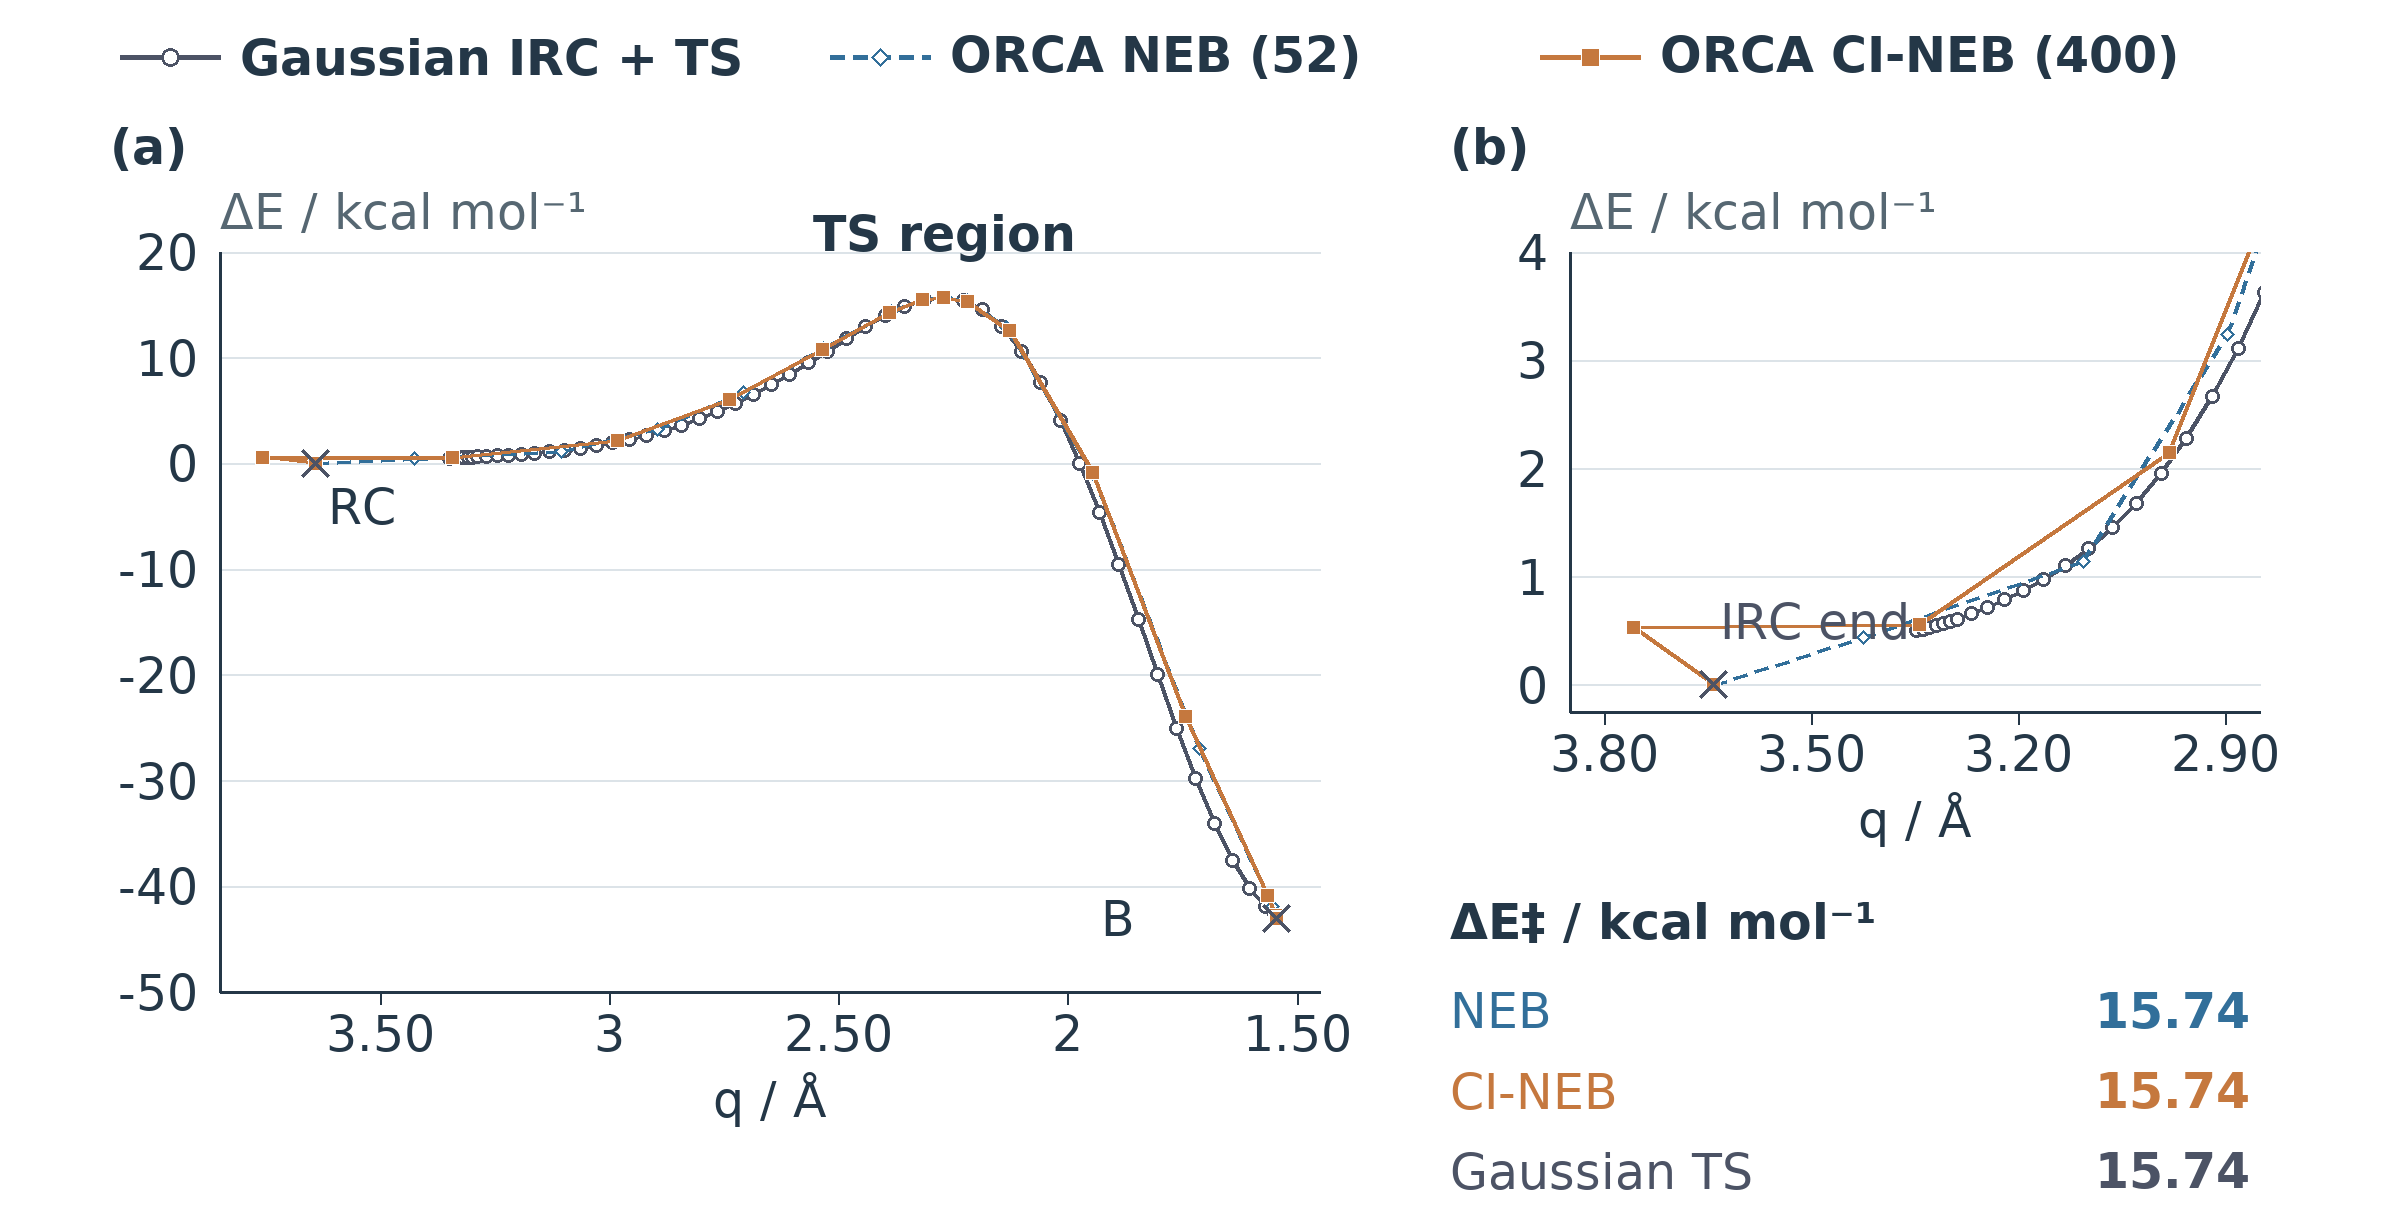
\includegraphics[width=\linewidth]{figures/neb-cineb-irc-comparison.png}
\caption{普通 NEB、CI-NEB 与 Gaussian IRC 的电子势能对照。零点分别取各程序的弱结合复合物；(a) 全路径，(b) 反应物侧放大。横轴 $q$ 为两条成键距离的平均值，是几何投影而非 IRC 坐标或 NEB 路径长度。折线按原顺序连接实际路径点，叉号为另行优化的 Gaussian 端点。IRC 使用原 TS，并非独立的第四次鞍点搜索；峰高接近不表示整条路径逐点重合。数值保留位数用于比较计算输出。}
\label{fig:path-comparison}
\end{figure}

\subsection{CI-NEB 峰顶的独立频率复核}
最终 CI-NEB 整带最大有效力为 $0.0186\ \mathrm{eV\,\AA^{-1}}$，达到采用的 $0.02\ \mathrm{eV\,\AA^{-1}}$ 标准。内部峰顶的真实最大原子力为 $3.13\times10^{-5}\ \mathrm{eV\,\AA^{-1}}$，已接近驻点。

独立数值频率包含 6 个平移、转动投影模式和 42 个振动模式，其中恰有一个 $516.1i\ \mathrm{cm^{-1}}$ 虚频。该模式使两条新键同时缩短，并伴随原双键伸长及 C2--C3 缩短（图~\ref{fig:cineb}）。保持共同碳编号、匹配等价氢并作正旋转配准后，新旧结构的全原子 RMSD 为 $9.12\times10^{-5}\ \mathrm{\AA}$，虚频位移的归一化内积绝对值为 $0.99998$。CI-NEB 与原 Gaussian TS 的几何和成键模式高度一致。

\begin{table}[htbp]
\centering\small
\caption{原 Gaussian TS 与 ORCA CI-NEB 峰顶的对照。频率均未缩放。}
\label{tab:cineb}
\begin{tabular}{lrr}
\toprule
量 & Gaussian TS & ORCA CI-NEB 峰顶\\
\midrule
C1--C5 / $\mathrm{\AA}$ & 2.271 & 2.271\\
C4--C6 / $\mathrm{\AA}$ & 2.271 & 2.271\\
唯一虚频 / $\mathrm{cm^{-1}}$ & $517.2i$ & $516.1i$\\
$E_{\rm el}$ / $E_{\rm h}$ & $-234.401776$ & $-234.401780$\\
$G$ / $E_{\rm h}$ & $-234.291876$ & $-234.291885$\\
\bottomrule
\end{tabular}
\end{table}

表~\ref{tab:cineb} 的 $G$ 为 $298.15\ \mathrm{K}$、$1\ \mathrm{atm}$ 下的 RRHO 值，峰顶转动对称数为 1。ORCA 采用 C/H 原子量 $12.011/1.008$，Gaussian 采用 $12.000/1.00782504$；两程序的频率微差包含原子质量约定和数值积分设置的影响\cite{orca-freq}。

\begin{figure}[htbp]
\centering
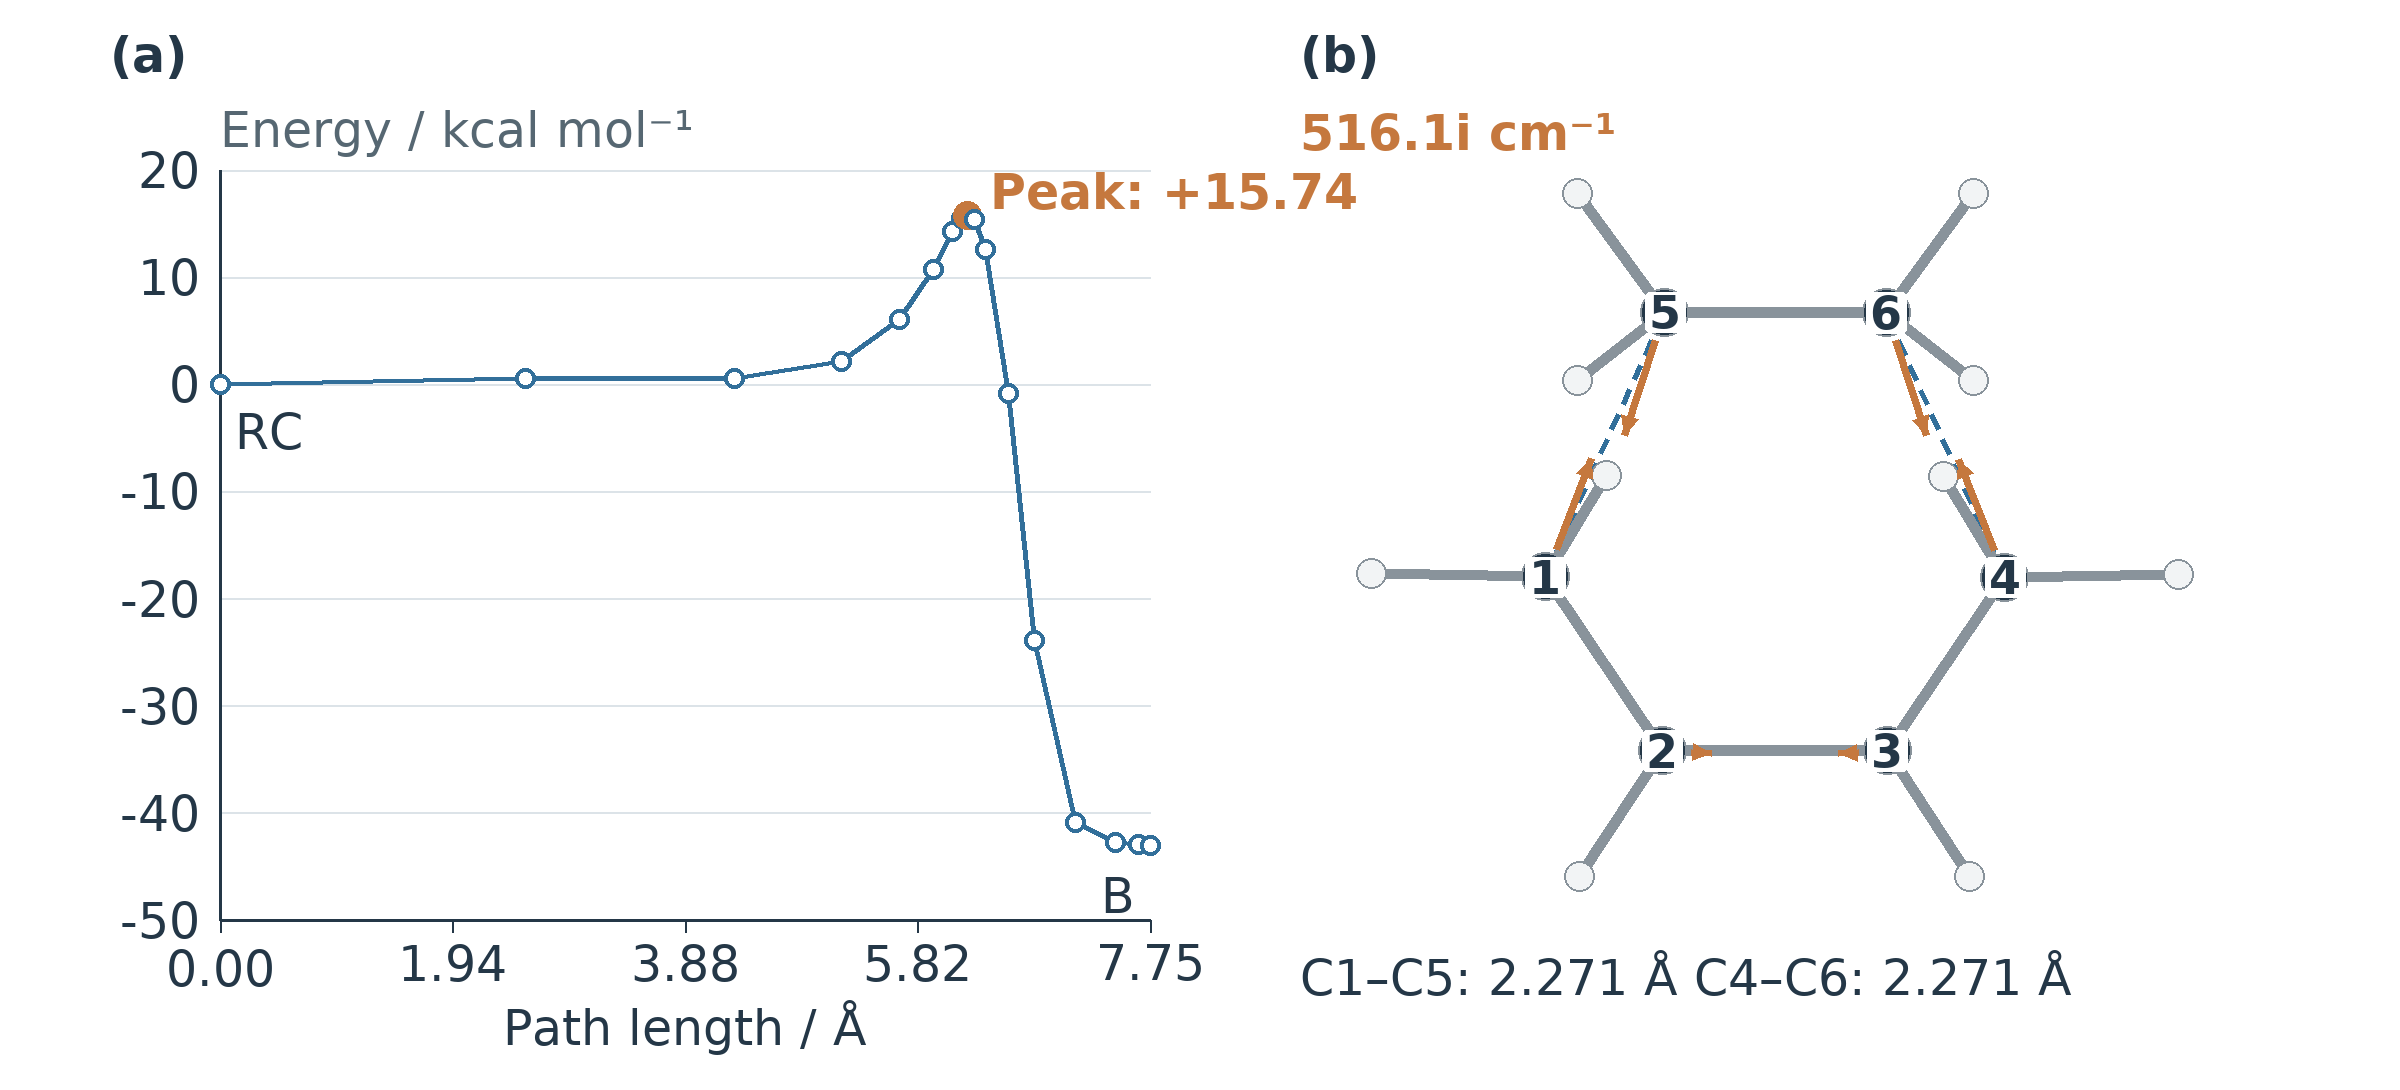
\includegraphics[width=\linewidth]{figures/cineb-ci400-review.png}
\caption{距离引导的 CI-NEB 电子势能与峰顶唯一虚频模式。(a) 17 个图像的电子能，零点为同带弱结合复合物，横轴为累计笛卡尔路径长度，折线仅连接计算图像；(b) 峰顶 $516.1i\ \mathrm{cm^{-1}}$ 模式，两条新键协同形成。整带最大有效力为 $0.0186\ \mathrm{eV\,\AA^{-1}}$，采用 $0.02$ 的标准。峰顶未另做 OptTS，经正旋转配准与原 Gaussian TS 的 RMSD 为 $0.000091\ \mathrm{\AA}$，模式重合为 $0.99998$。此图为电子势能路径，不是 IRC 或自由能曲线。}
\label{fig:cineb}
\end{figure}

\subsection{电子能与 Gibbs 自由能}
Gaussian 各驻点的电子能和自由能列于表~\ref{tab:absolute}。原始自由能 $G_{\rm out}$ 与式~\eqref{eq:sigma} 的对称数修正结果分别列出。

\begin{table}[htbp]
\centering\footnotesize
\caption{各驻点的绝对能量（Hartree）。$G$ 为转动对称数修正后的值。}
\label{tab:absolute}
\setlength{\tabcolsep}{4pt}
\begin{tabular}{lrrr}
\toprule
体系 & $E_{\rm el}$ & $G_{\rm out}$ & $G$\\
\midrule
乙烯 & $-78.535525$ & $-78.505711$ & $-78.505711$\\
丁二烯 & $-155.886887$ & $-155.829001$ & $-155.828347$\\
反应物复合物 & $-234.426861$ & $-234.327318$ & $-234.327318$\\
环加成 TS & $-234.401776$ & $-234.291876$ & $-234.291876$\\
环己烯 B & $-234.495414$ & $-234.379714$ & $-234.379714$\\
环己烯 A & $-234.504281$ & $-234.387199$ & $-234.386545$\\
\bottomrule
\end{tabular}
\end{table}

\begin{table}[htbp]
\centering\small
\caption{相对于两个分离反应物的能量差（$\kcalmol$）。每列采用相应的反应物能量之和为零点。}
\label{tab:relative}
\setlength{\tabcolsep}{4pt}
\begin{tabular}{lrrrrr}
\toprule
体系 & $\Delta E_{\rm el}$ & $\Delta(E+\mathrm{ZPE})$ & $\Delta H$ & $\Delta G_{\rm out}$ & $\Delta G$\\
\midrule
反应物复合物 & $-2.79$ & $-2.09$ & $-1.50$ & $4.64$ & $4.23$\\
环加成 TS & $12.95$ & $15.51$ & $14.07$ & $26.88$ & $26.47$\\
环己烯 B & $-45.81$ & $-39.48$ & $-41.30$ & $-28.24$ & $-28.65$\\
环己烯 A & $-51.37$ & $-44.89$ & $-46.91$ & $-32.94$ & $-32.94$\\
\bottomrule
\end{tabular}
\end{table}

环加成的电子能垒为 $12.95\ \kcalmol$，加入零点校正后为 $15.51\ \kcalmol$，活化自由能为 $26.47\ \kcalmol$。由 $\Delta G^{\ddagger}=\Delta H^{\ddagger}-T\Delta S^{\ddagger}$ 得 $\Delta S^{\ddagger}\approx-41.60\ \mathrm{cal\,mol^{-1}\,K^{-1}}$；两个分离分子形成一个受限的活化复合体，熵降低使自由能垒显著高于焓垒。

生成 IRC 直接连接的 B 时，反应自由能为 $-28.65\ \kcalmol$；独立优化构象 A 的相对自由能为 $-32.94\ \kcalmol$。反应物复合物的电子能比两个分离反应物低 $2.79\ \kcalmol$，但其自由能高 $4.23\ \kcalmol$，说明电子结合与标准态下缔合的自由能变化并不等同。图~\ref{fig:gibbs} 保持分离反应物为零点。

\begin{figure}[htbp]
\centering
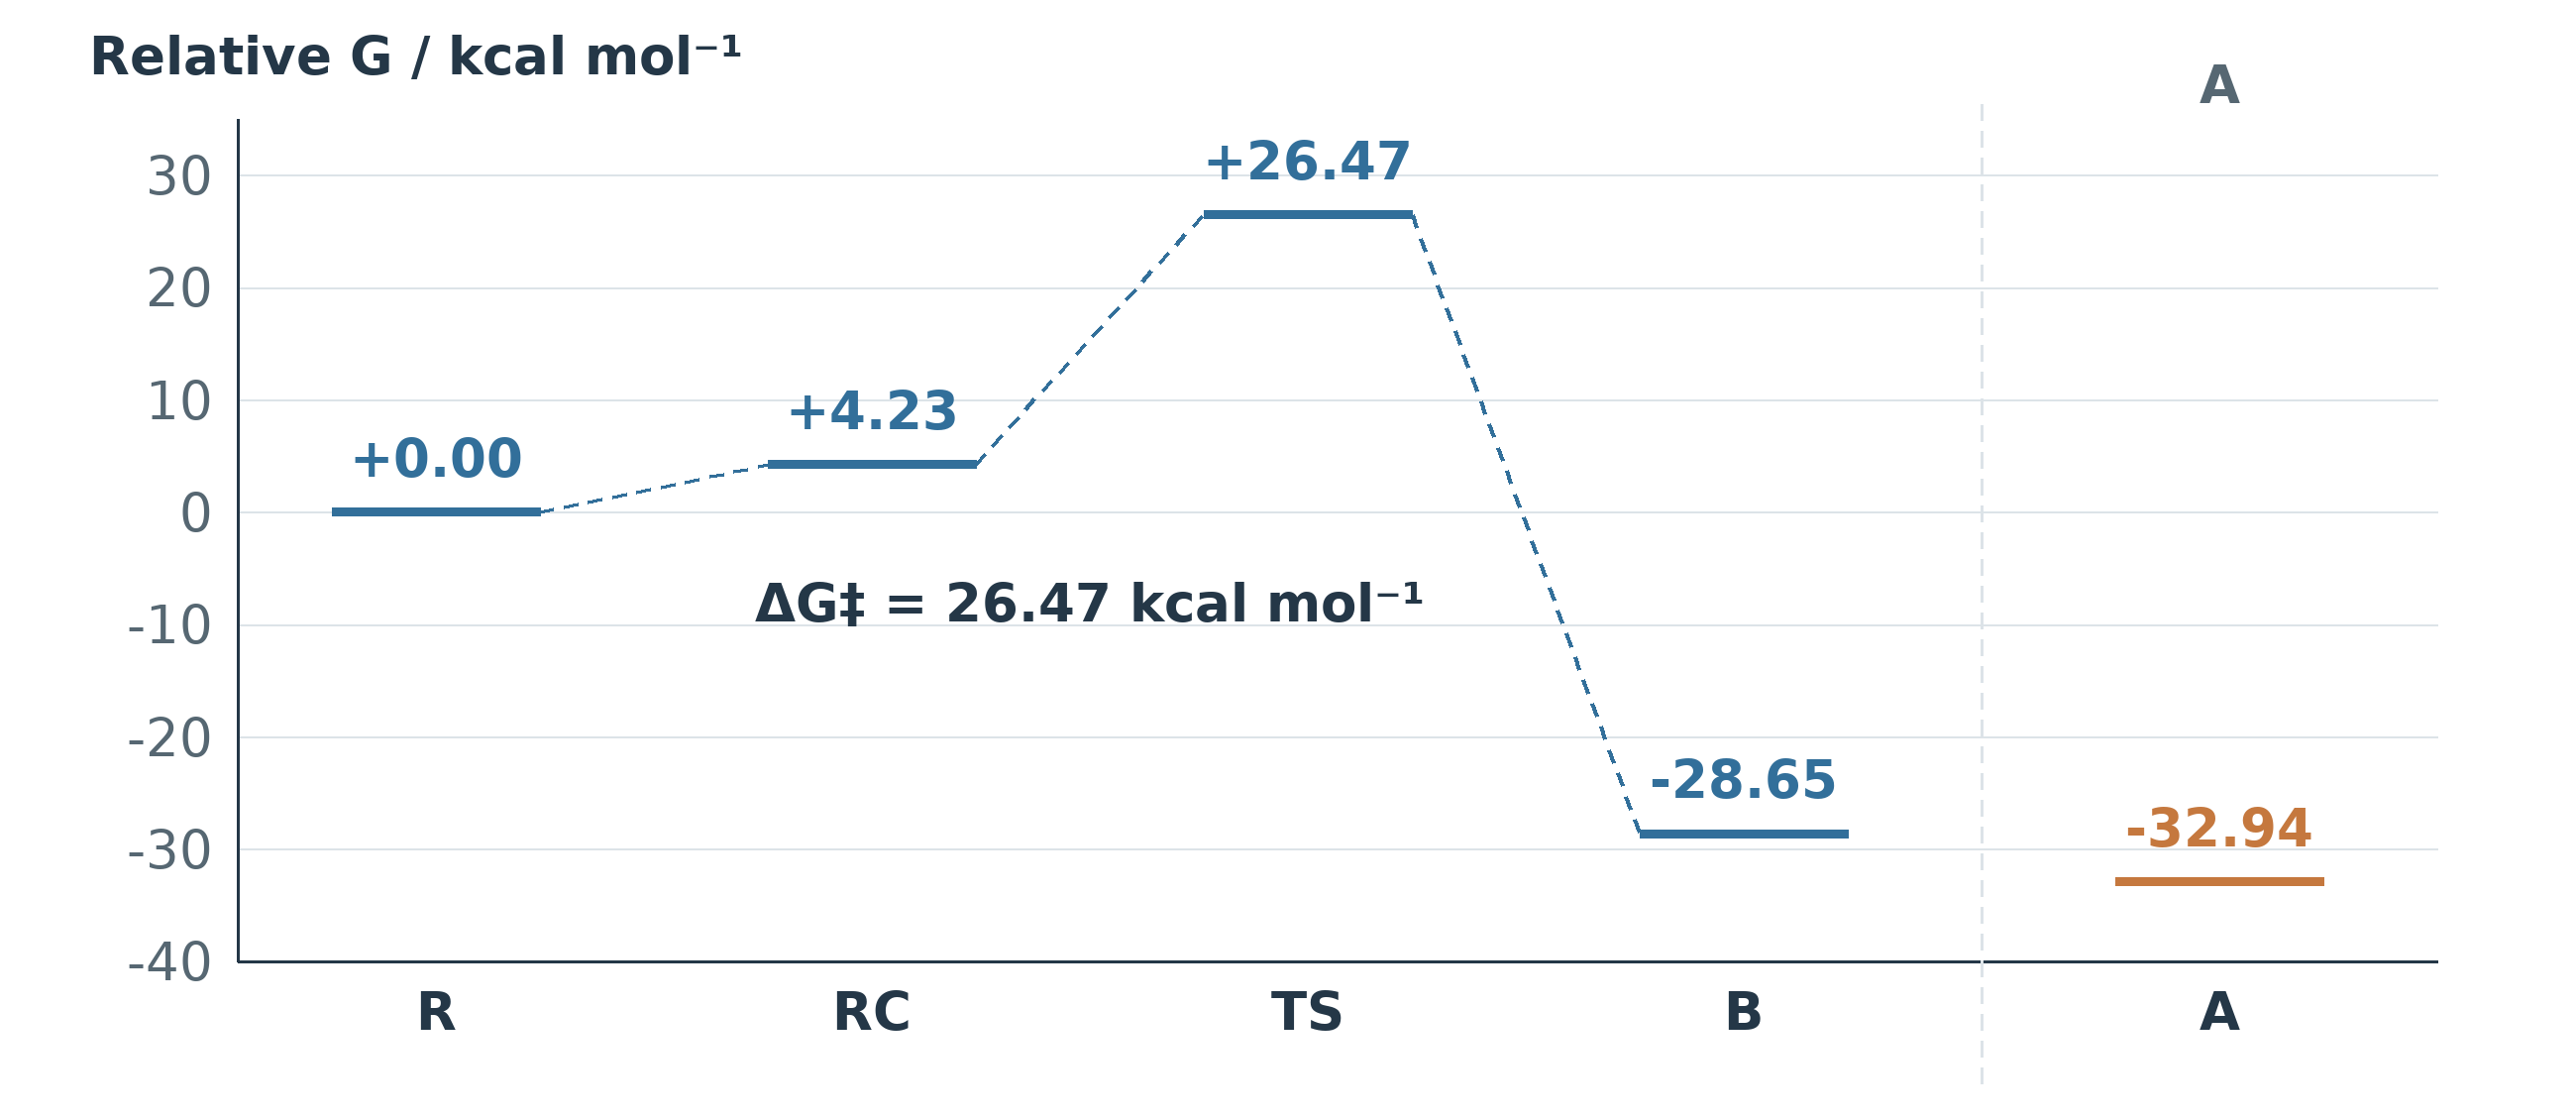
\includegraphics[width=\linewidth]{figures/gibbs-free-energy-profile.png}
\caption{$298.15\ \mathrm{K}$、$1\ \mathrm{atm}$ 下经转动对称数修正的 RRHO Gibbs 自由能，以孤立丁二烯和乙烯之和为零点，各物种采用一个构象。丁二烯二面角为 $26.9^\circ$；B 为 IRC 连接的产物，A 单列比较稳定性，不在此图连接 A/B。虚线仅引导离散能级的阅读，不表示 IRC 电子能或连续自由能路径。}
\label{fig:gibbs}
\end{figure}

热化学比较采用同一 RRHO 处理。B 的 $45.46\ \mathrm{cm^{-1}}$ 模式主要是环扭转，复合物低于 $100\ \mathrm{cm^{-1}}$ 的五个模式主要是碎片间平移与转动。这些软模式的谐振子熵对低频处理较敏感，因此小幅自由能差也更依赖这一处理。

\subsection{前线轨道与成键相位}
由独立优化反应物的波函数绘制丁二烯 HOMO（MO 15）和乙烯 LUMO（MO 9），等值面统一取 $\pm0.030\ \mathrm{bohr^{-3/2}}$（图~\ref{fig:orbitals}）。颜色表示波函数正负号，不表示正负电荷；单个轨道的整体符号可任意反转，具有物理意义的是不同位置之间的相对相位。

\begin{figure}[htbp]
\centering
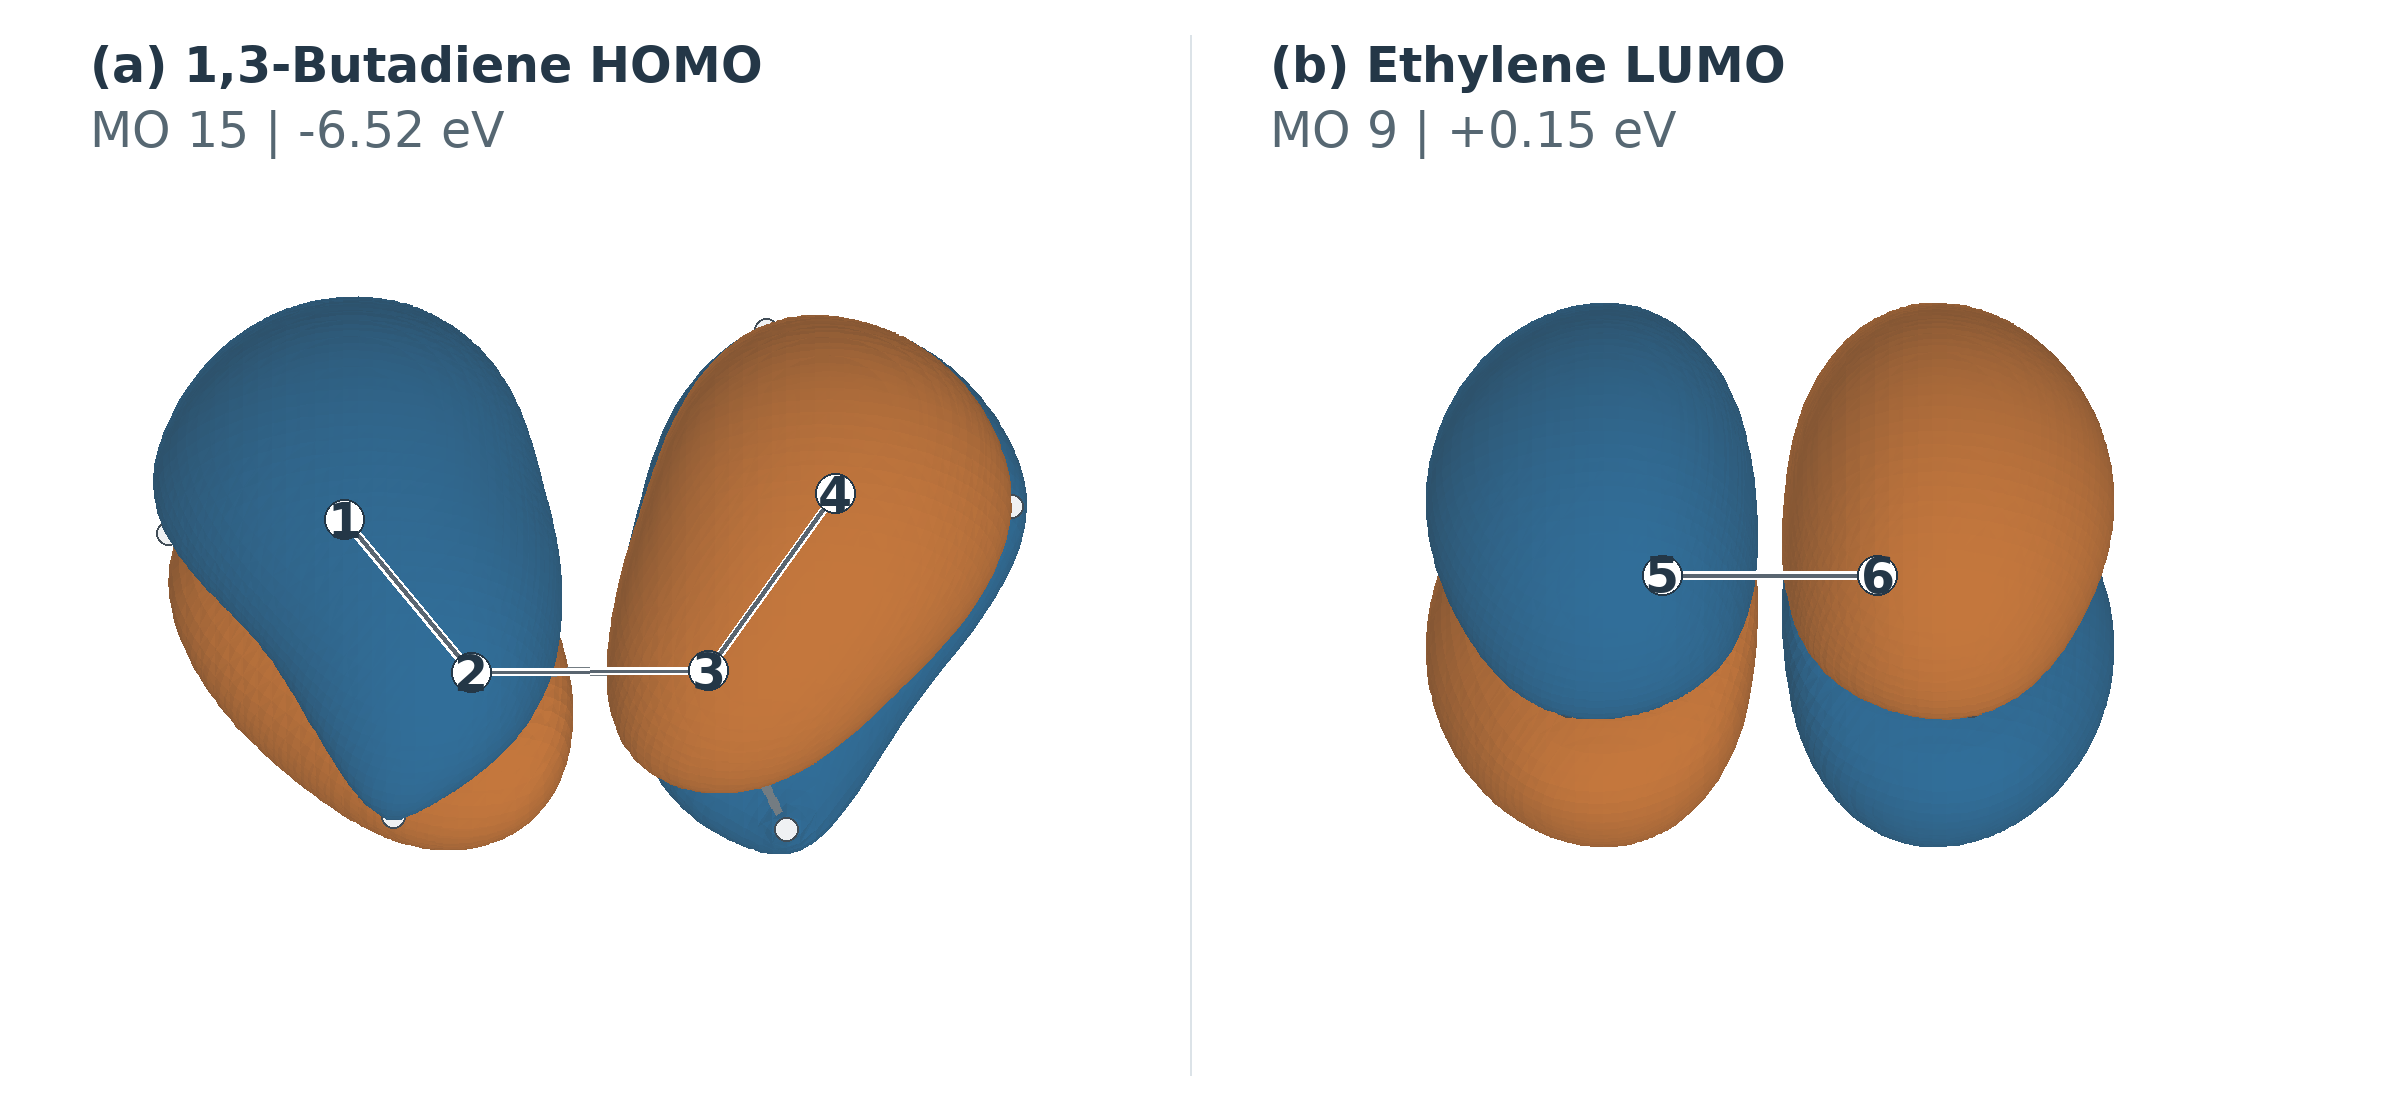
\includegraphics[width=\linewidth]{figures/frontier-orbital-surfaces.png}
\caption{丁二烯 HOMO 与乙烯 LUMO 的真实波函数等值面，来自各自优化的孤立分子，采用相同空间尺度及 $\pm0.030\ \mathrm{bohr^{-3/2}}$ 阈值。蓝、橙色分别表示正、负相位，整体符号任意；编号碳骨架用于标明取向。丁二烯二面角为 $26.90^\circ$，乙烯 LUMO 为反键 $\pi^*$ 轨道。}
\label{fig:orbitals}
\end{figure}

将孤立反应物的片段轨道按照 TS 中的相对朝向刚性排列后，两条接近方向 C1--C5 与 C4--C6 上均可实现同相重叠（图~\ref{fig:phase}）。这一相位关系使两个端点同时产生有利的成键相互作用，与频率及 IRC 所揭示的协同成键相一致。

\begin{figure}[htbp]
\centering
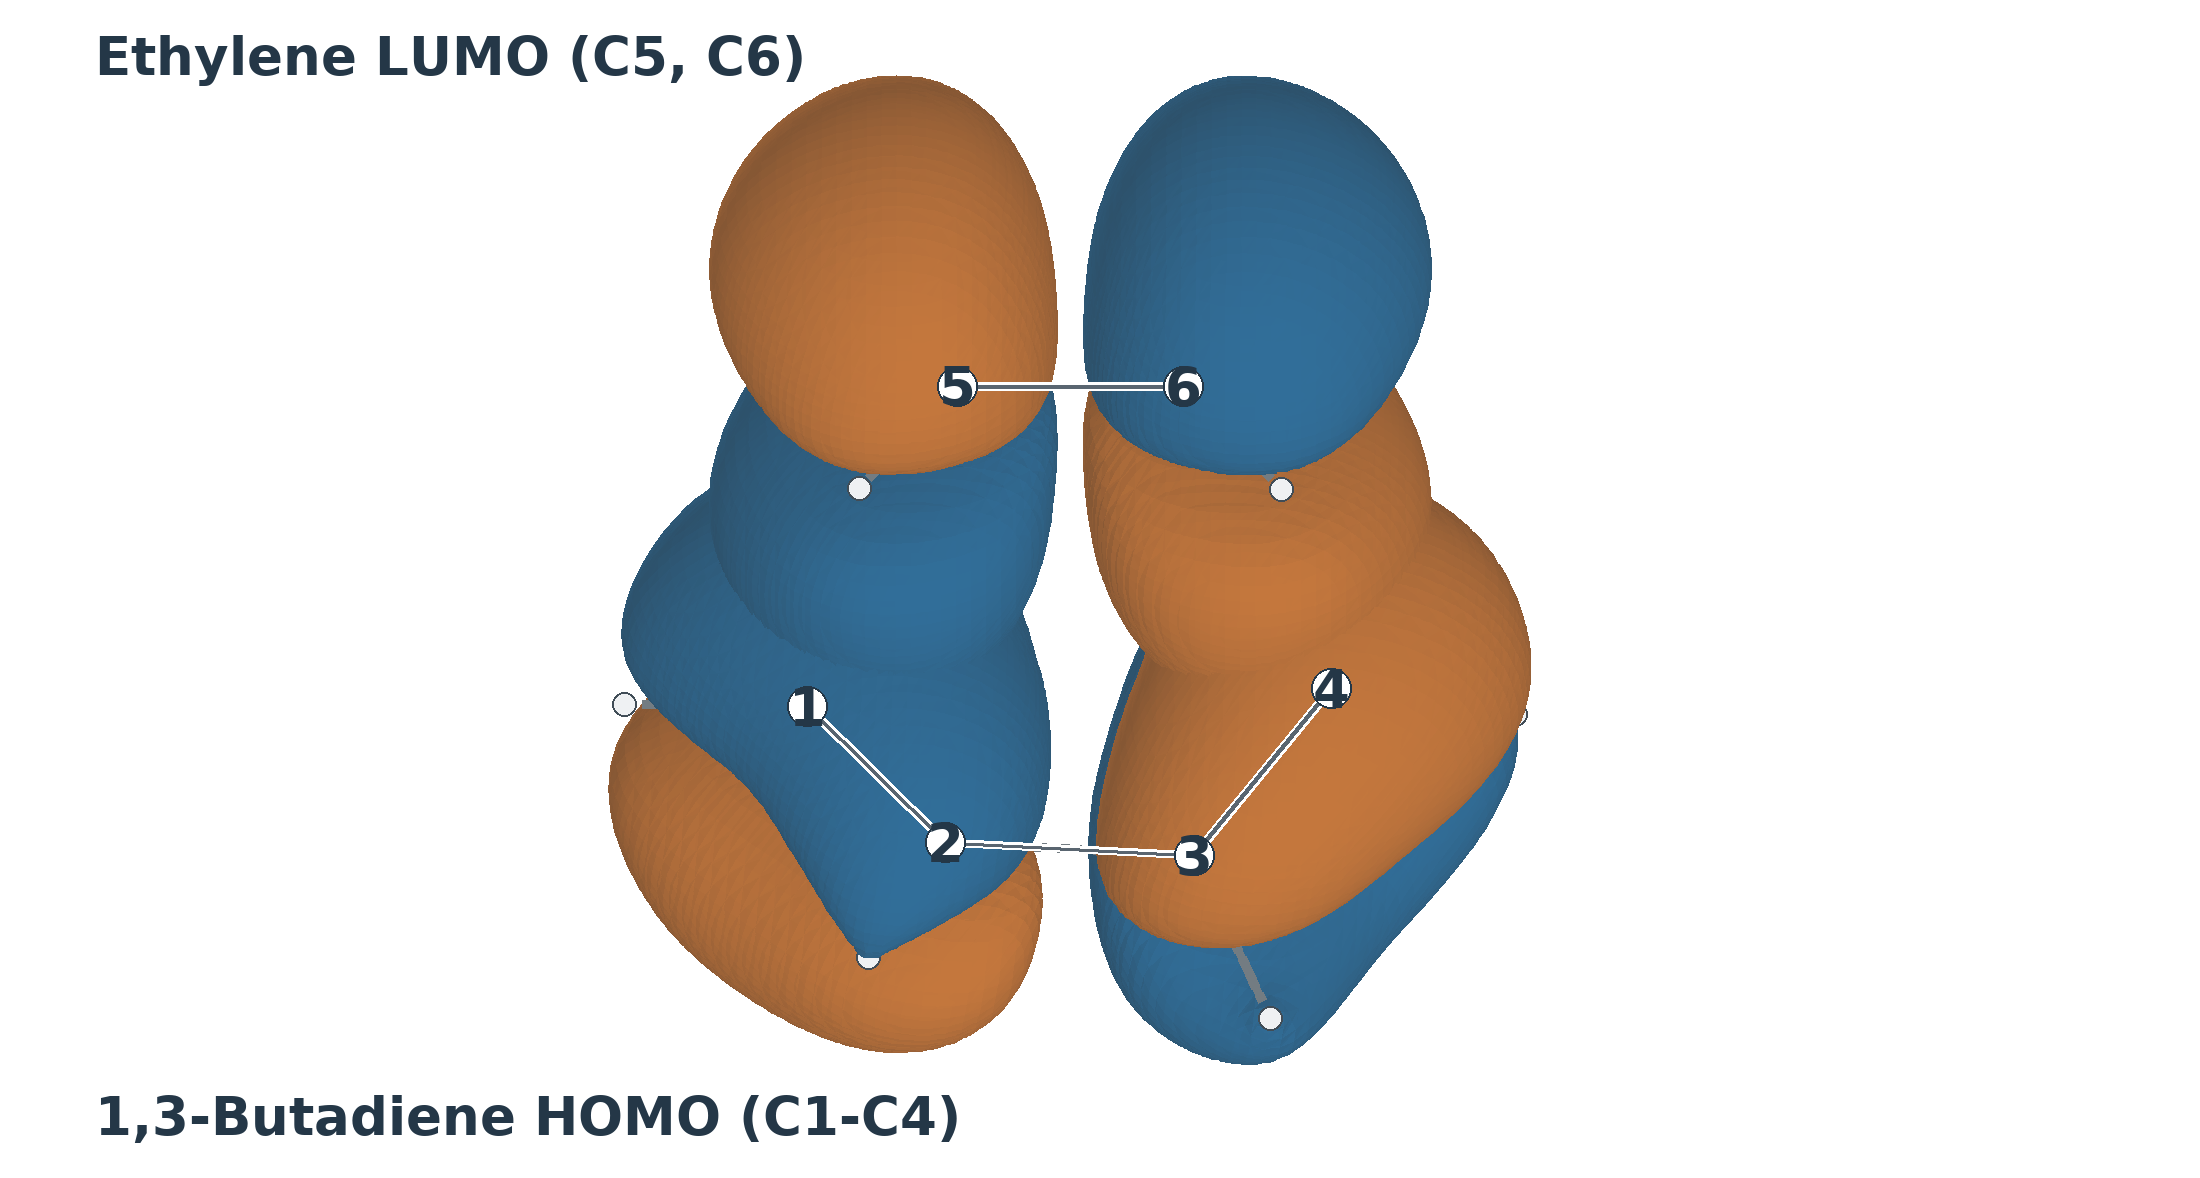
\includegraphics[width=0.84\linewidth]{figures/frontier-phase-matching.png}
\caption{沿 C1--C5、C4--C6 两条成键接近方向比较片段轨道相位，两处相向叶瓣均可同相。等值面阈值为 $\pm0.030\ \mathrm{bohr^{-3/2}}$；仅平移、旋转孤立片段到 TS 的接近朝向，保持其优化几何与波函数。乙烯轨道整体换号不改变物理结果；所示为片段轨道比较，而非 TS 的分子轨道。}
\label{fig:phase}
\end{figure}

丁二烯 HOMO 能量为 $-6.52\ \mathrm{eV}$，乙烯 LUMO 为 $+0.15\ \mathrm{eV}$，两者相差 $6.67\ \mathrm{eV}$。反向的乙烯 HOMO--丁二烯 LUMO 能隙约为 $6.52\ \mathrm{eV}$，两组能隙接近，说明两个方向的供受体相互作用均值得考虑。轨道能级见图~\ref{fig:levels}。

\begin{figure}[htbp]
\centering
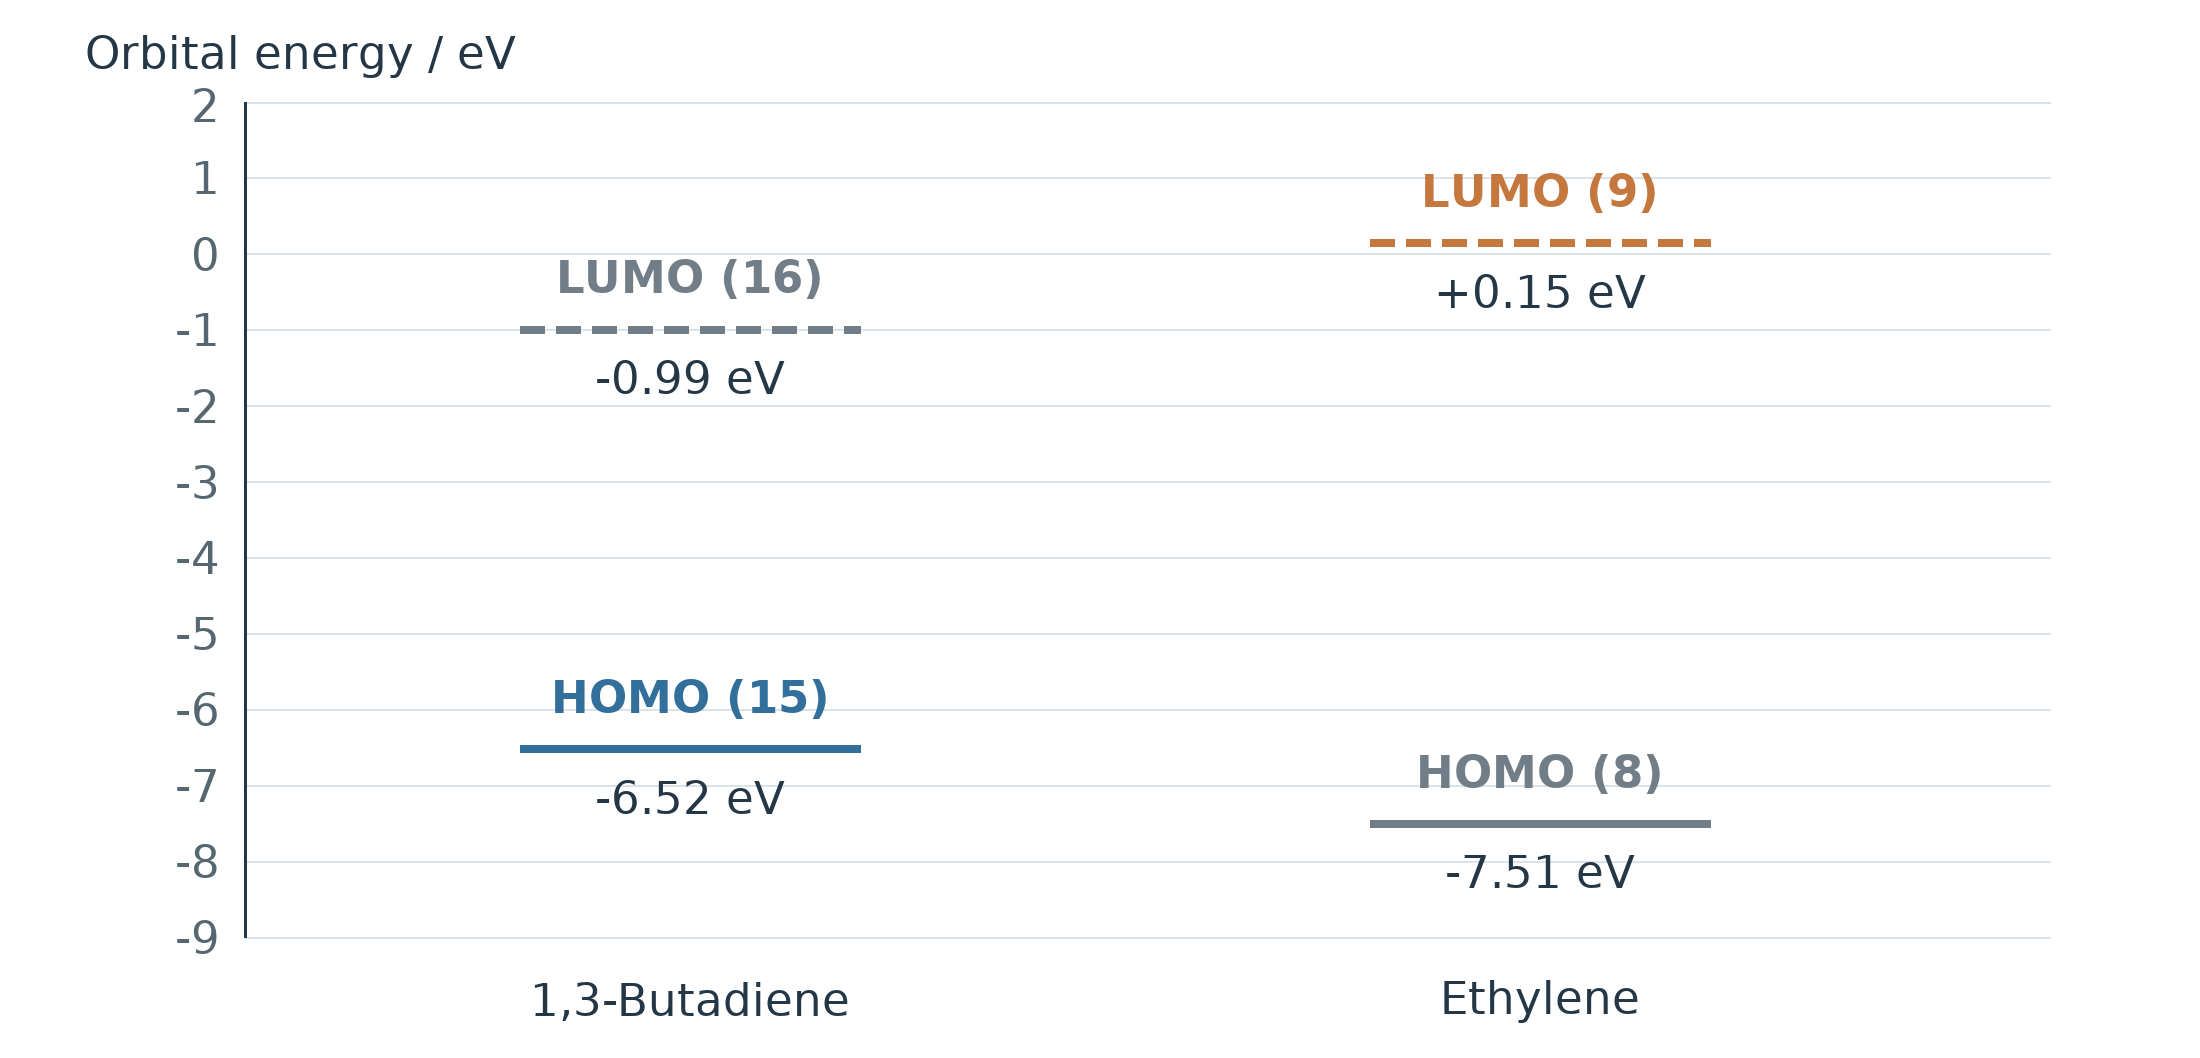
\includegraphics[width=\linewidth]{figures/frontier-orbital-levels.png}
\caption{孤立优化反应物的前线轨道能级。实线为占据轨道，虚线为未占据轨道；轨道本征值之差不是活化能或激发能。}
\label{fig:levels}
\end{figure}

\subsection{环己烯构象比较}
构象 A 与 B 均为无虚频的局部极小值。B 的电子能比 A 高 $5.56\ \kcalmol$，对称数修正后的自由能高 $4.29\ \kcalmol$。它们具有相同共价连接关系，主要差异为六元环的空间扭曲。

以两种构象进行 QST2 搜索，得到一个环扭转一阶鞍点，其 42 个振动模式中有唯一的 $66.2i\ \mathrm{cm^{-1}}$ 虚频，位移主要改变环二面角。该鞍点相对于 A、B 的能量高度列于表~\ref{tab:conformer}。

\begin{table}[htbp]
\centering\small
\caption{Gaussian 环扭转鞍点相对构象 A、B 的能量高度（$\kcalmol$）。}
\label{tab:conformer}
\begin{tabular}{lrrrr}
\toprule
参考构象 & $\Delta E_{\rm el}$ & $\Delta(E+\mathrm{ZPE})$ & $\Delta G_{\rm out}$ & $\Delta G$\\
\midrule
A & $5.59$ & $5.34$ & $5.59$ & $5.17$\\
B & $0.028$ & $-0.065$ & $0.89$ & $0.89$\\
\bottomrule
\end{tabular}
\end{table}
B 一侧的电子能高度仅 $0.028\ \kcalmol$，零点校正后鞍点能级略低于 B，显示该区域势能面非常平缓。这一级别的能量差对低频振动和零点校正尤为敏感。

端点独立构建的 ORCA 路径中，普通 NEB 在第 35 步达到整带最大有效力 $0.0493\ \mathrm{eV\,\AA^{-1}}$，CI-NEB 在第 50 步达到 $0.00676\ \mathrm{eV\,\AA^{-1}}$。以同一组 ORCA 优化端点的电子能为参考，普通 NEB、CI-NEB 及精修鞍点相对 A 的高度依次为 $5.83$、$5.59$、$5.59\ \kcalmol$，相对 B 则为 $0.26$、$0.028$、$0.027\ \kcalmol$。CI-NEB 显著降低了普通 NEB 峰顶的残余能量，随后 OptTS 精修仅带来很小的变化。

精修结构具有唯一的 $67.6i\ \mathrm{cm^{-1}}$ 环扭转虚频，真实最大残余力为 $9.98\times10^{-5}\ \mathrm{eV\,\AA^{-1}}$。保持碳编号、匹配等价氢并作正旋转配准后，与 Gaussian 构象鞍点的全原子 RMSD 为 $0.0021\ \mathrm{\AA}$，虚频模式重合度为 $0.99998$。两种搜索得到了高度一致的环扭转鞍点，均显示 B 一侧势垒很浅。A/B 路径由收敛的 CI-NEB 支持；构象双向 IRC 未完成。

\begin{figure}[htbp]
\centering
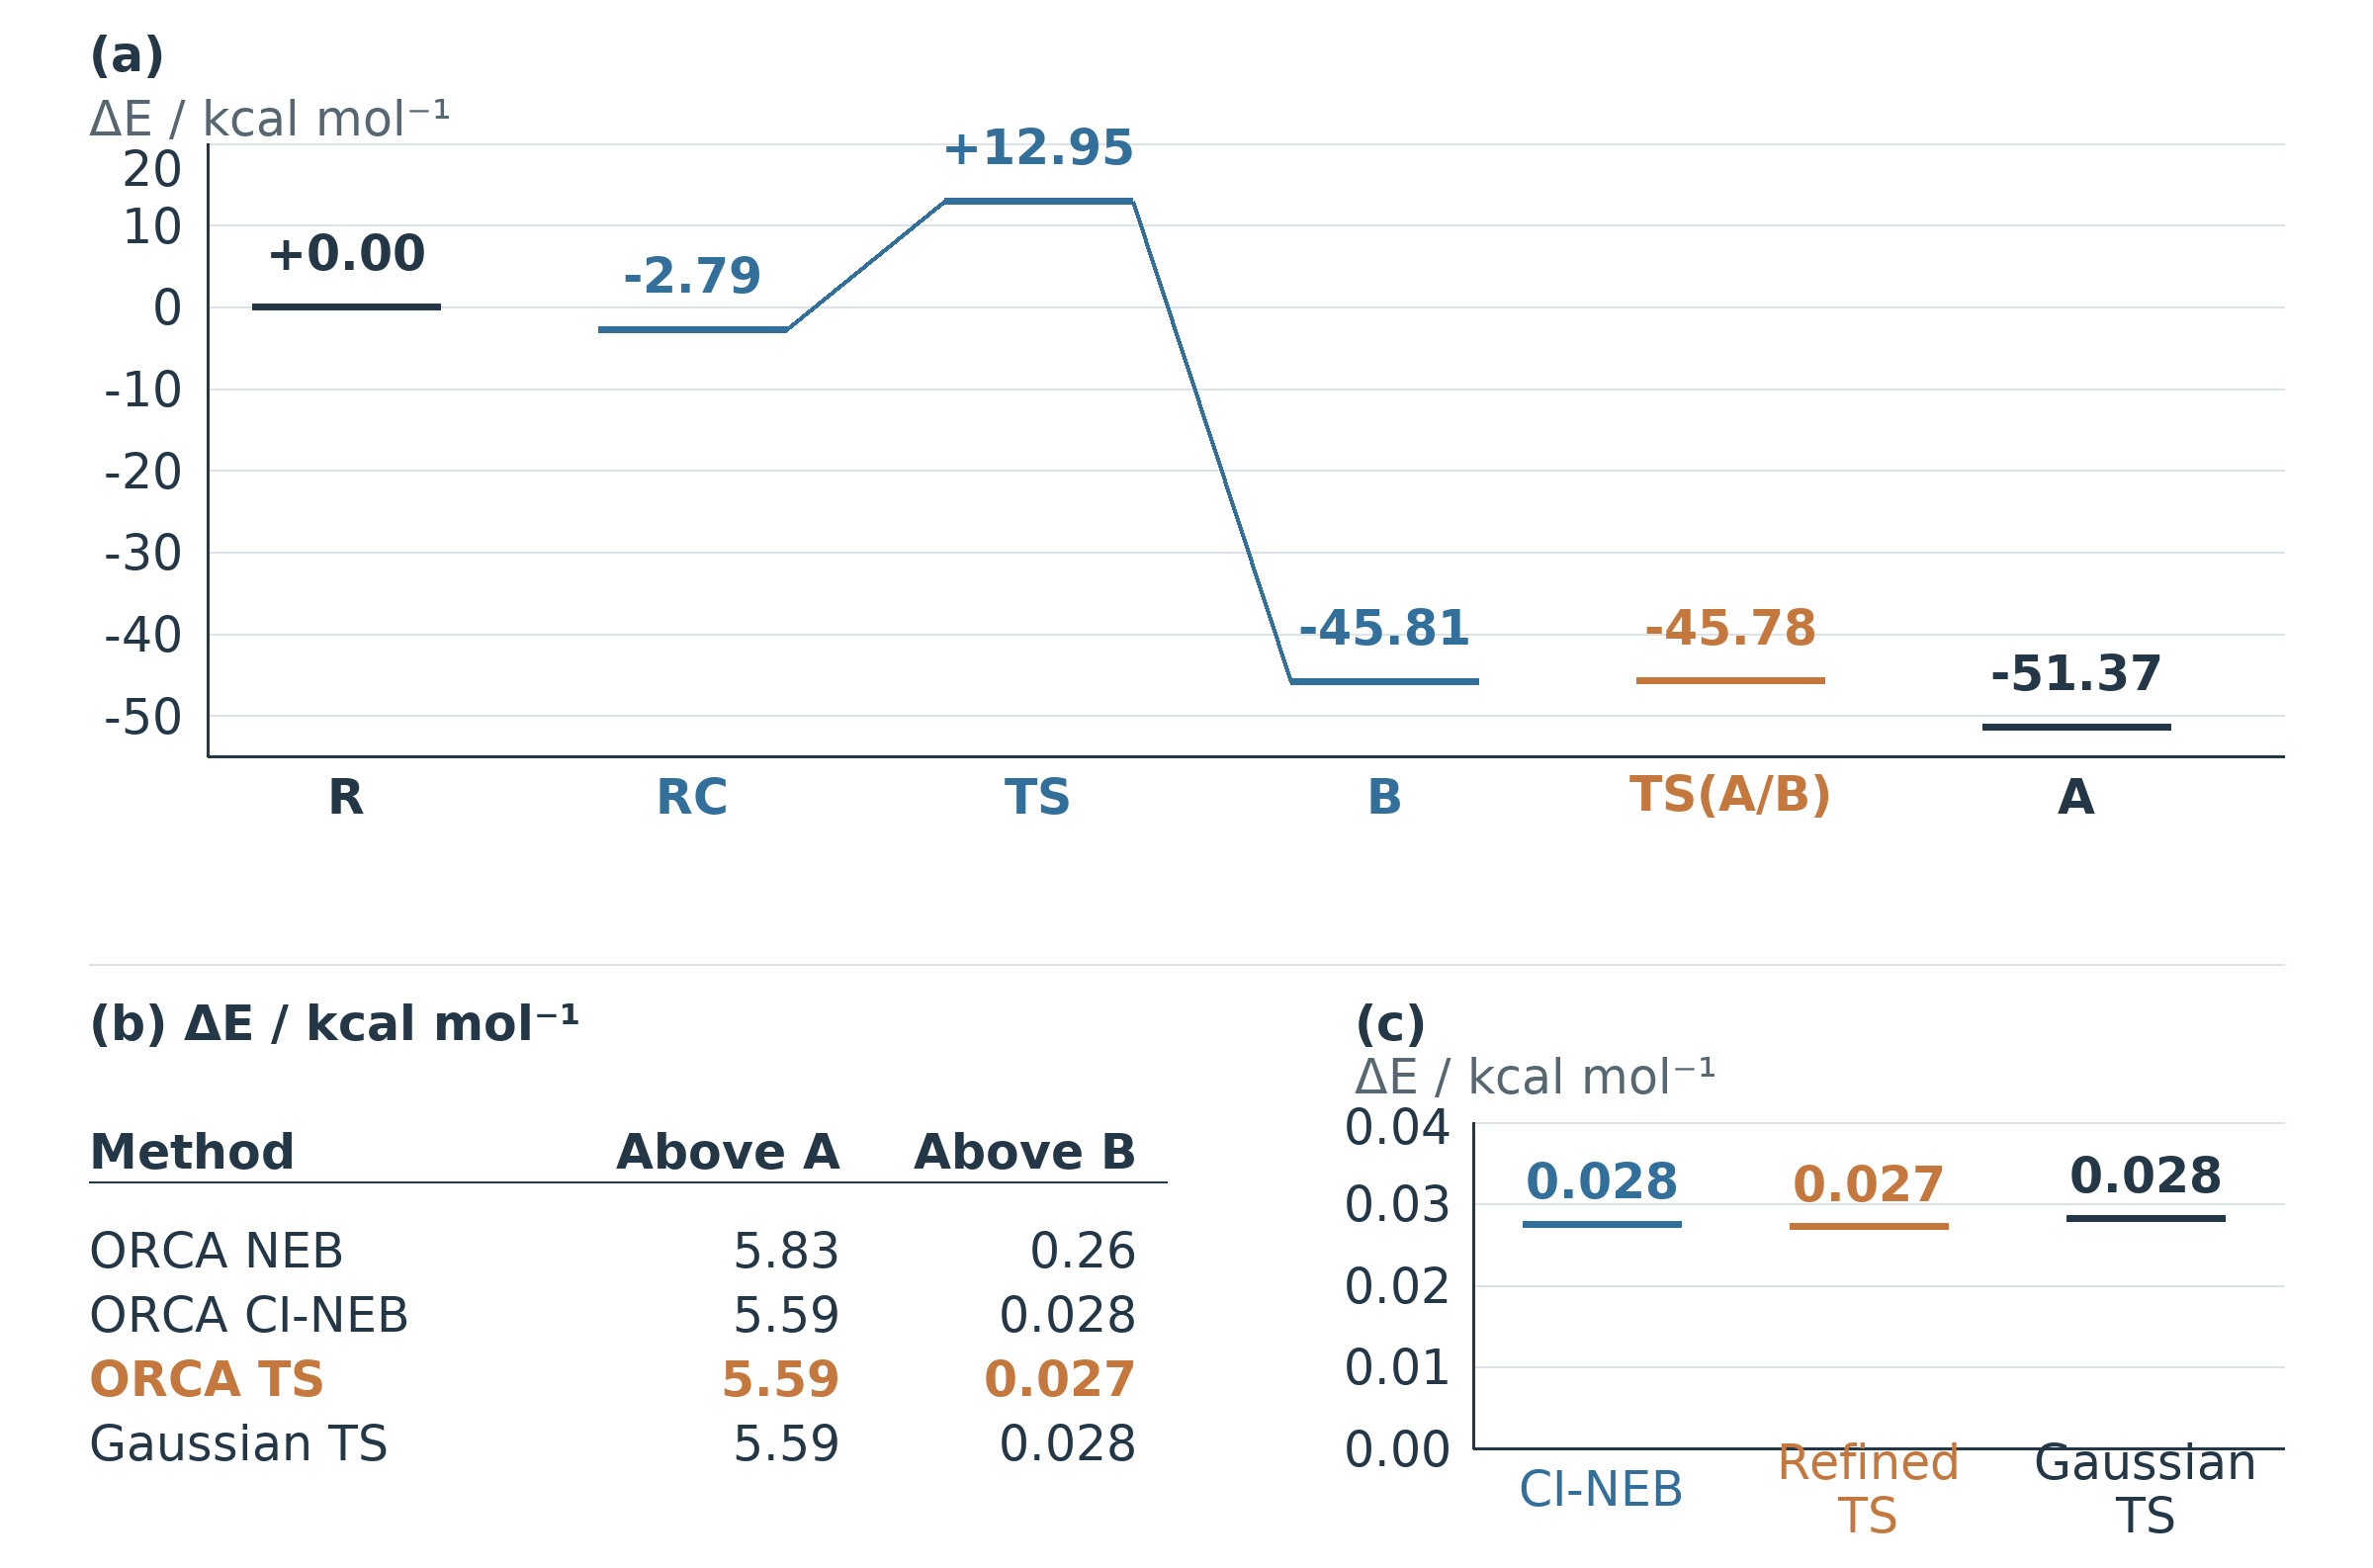
\includegraphics[width=\linewidth]{figures/electronic-energy-ladder-complete.png}
\caption{完整电子能阶梯及构象鞍点对照。(a) Gaussian 能级，以分离反应物为零点，实线连接 IRC 确认的 RC--TS--B；A/B 鞍点与 B 近简并，未画出尚未确认的双向连接。(b) 各程序以自身优化端点为参考的峰高，ORCA 各行统一采用端点频率计算的电子能；精修鞍点具有唯一 $67.6i\ \mathrm{cm^{-1}}$ 环扭转模式。(c) B 侧能级放大，其微小高度不用于推算精确速率。全部为未加零点能和热校正的离散电子能，横向间隔为示意。}
\label{fig:energy-ladder-complete}
\end{figure}

\subsection{1,3-丁二烯与顺丁烯二酸酐的环加成}
沿用相同物理模型，进一步研究 1,3-丁二烯与顺丁烯二酸酐生成顺式加成产物的反应。该体系为 $\mathrm{C_8H_8O_3}$，含 19 个原子、80 个电子和 51 个振动模式。丁二烯的四个碳记为 C1--C4，酸酐的两个烯碳为 C5、C6；反应形成 C1--C5、C4--C6，产物保留 C2=C3。各程序均独立优化反应物、过渡态和产物，丁二烯采用本次优化的近 s-cis 扭曲构象作为参照。

现有路径为 endo 进攻：过渡态中酸酐部分朝向丁二烯的 C2、C3 内侧。Gaussian 过渡态两条形成键均约为 $2.262\ \mathrm{\AA}$，51 个振动中唯一虚频为 $443.0i\ \mathrm{cm^{-1}}$，对应两端协同成键。ORCA 过渡态的相应虚频为 $443.0i\ \mathrm{cm^{-1}}$，正旋转与等价氢匹配后的全原子 RMSD 为 $0.00014\ \mathrm{\AA}$，模式重合度为 $0.99999$。两套计算给出高度一致的局部过渡态结构和运动。

\begin{figure}[htbp]
\centering
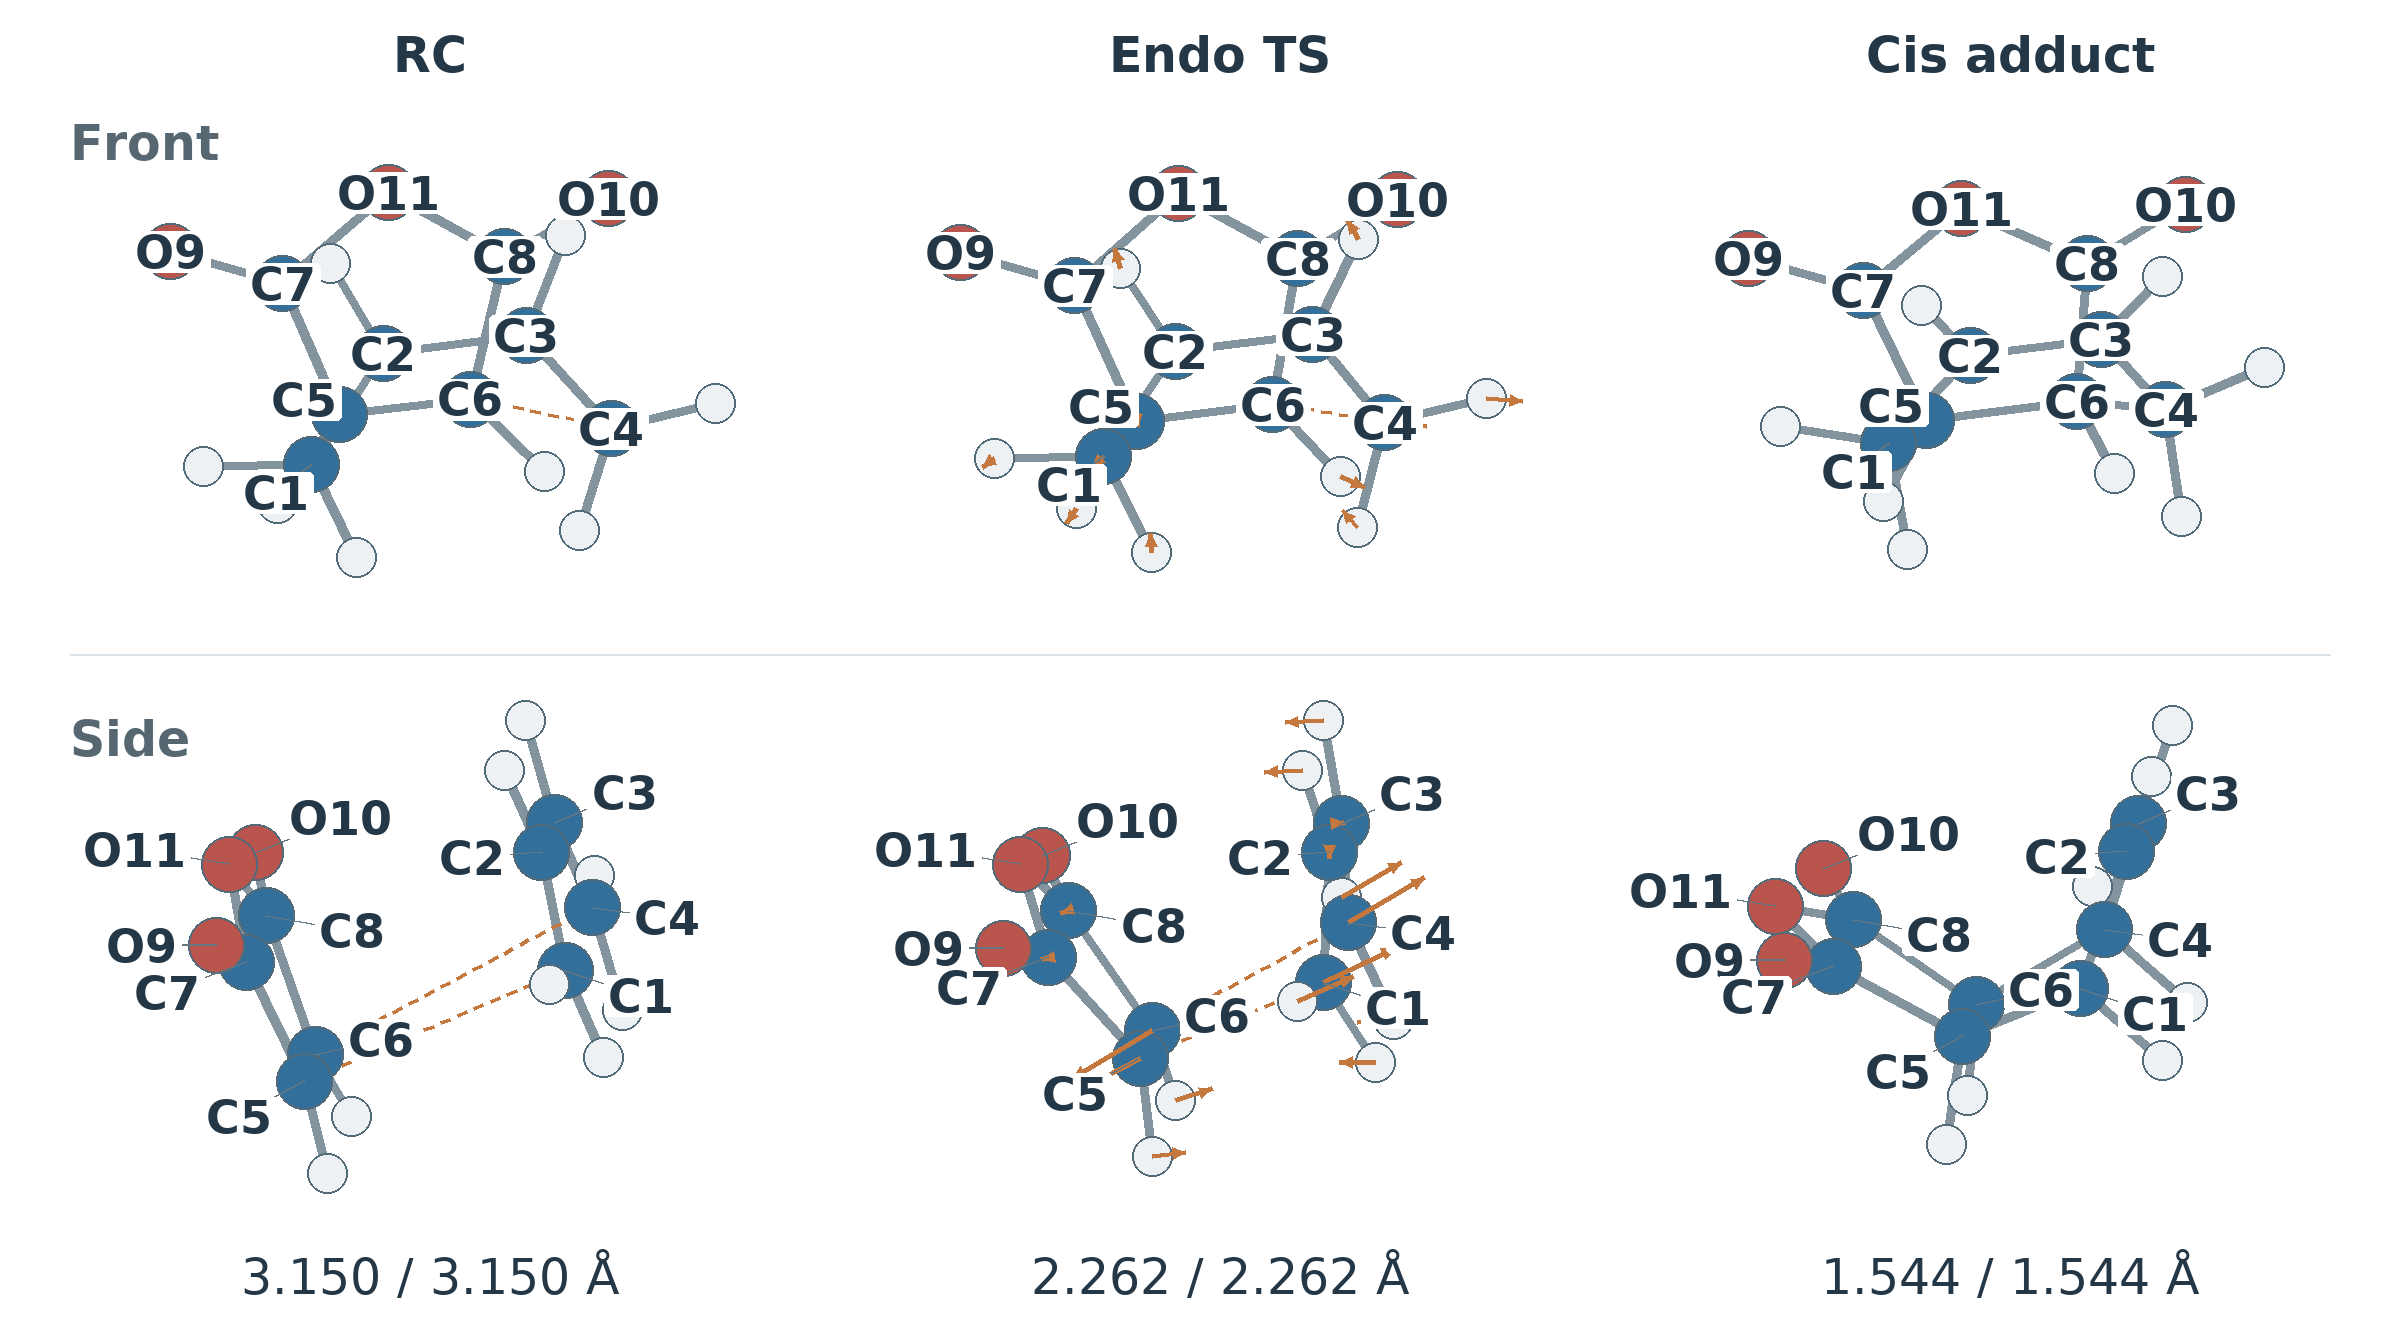
\includegraphics[width=\linewidth]{figures/maleic-structures-multiview.png}
\caption{endo 路径的 Gaussian 反应物复合物、环加成过渡态及顺式产物。上、下两排分别为统一观察方向的正视和侧视图，同一列使用同一优化结构；侧视图显示酸酐部分与丁二烯的相对朝向。蓝、红、浅灰原子分别为 C、O、H；标注数值依次为 C1--C5、C4--C6 距离。橙色箭头表示唯一 $443.0i\ \mathrm{cm^{-1}}$ 虚频的位移方向。}
\label{fig:maleic-structures}
\end{figure}

Gaussian 双向 IRC 在反应物侧得到 22 个收敛点，在产物侧得到 30 个收敛点。沿路径两条新键几乎同步缩短（图~\ref{fig:maleic-irc}）。两端继续优化后分别得到反应物复合物和顺式产物，均有 51 个实频；两条新键距离分别为 $3.150$、$1.544\ \mathrm{\AA}$。IRC 产物与独立优化产物的 RMSD 为 $0.00083\ \mathrm{\AA}$，电子能差仅 $0.0014\ \kcalmol$，属于同一构象。

\begin{figure}[htbp]
\centering
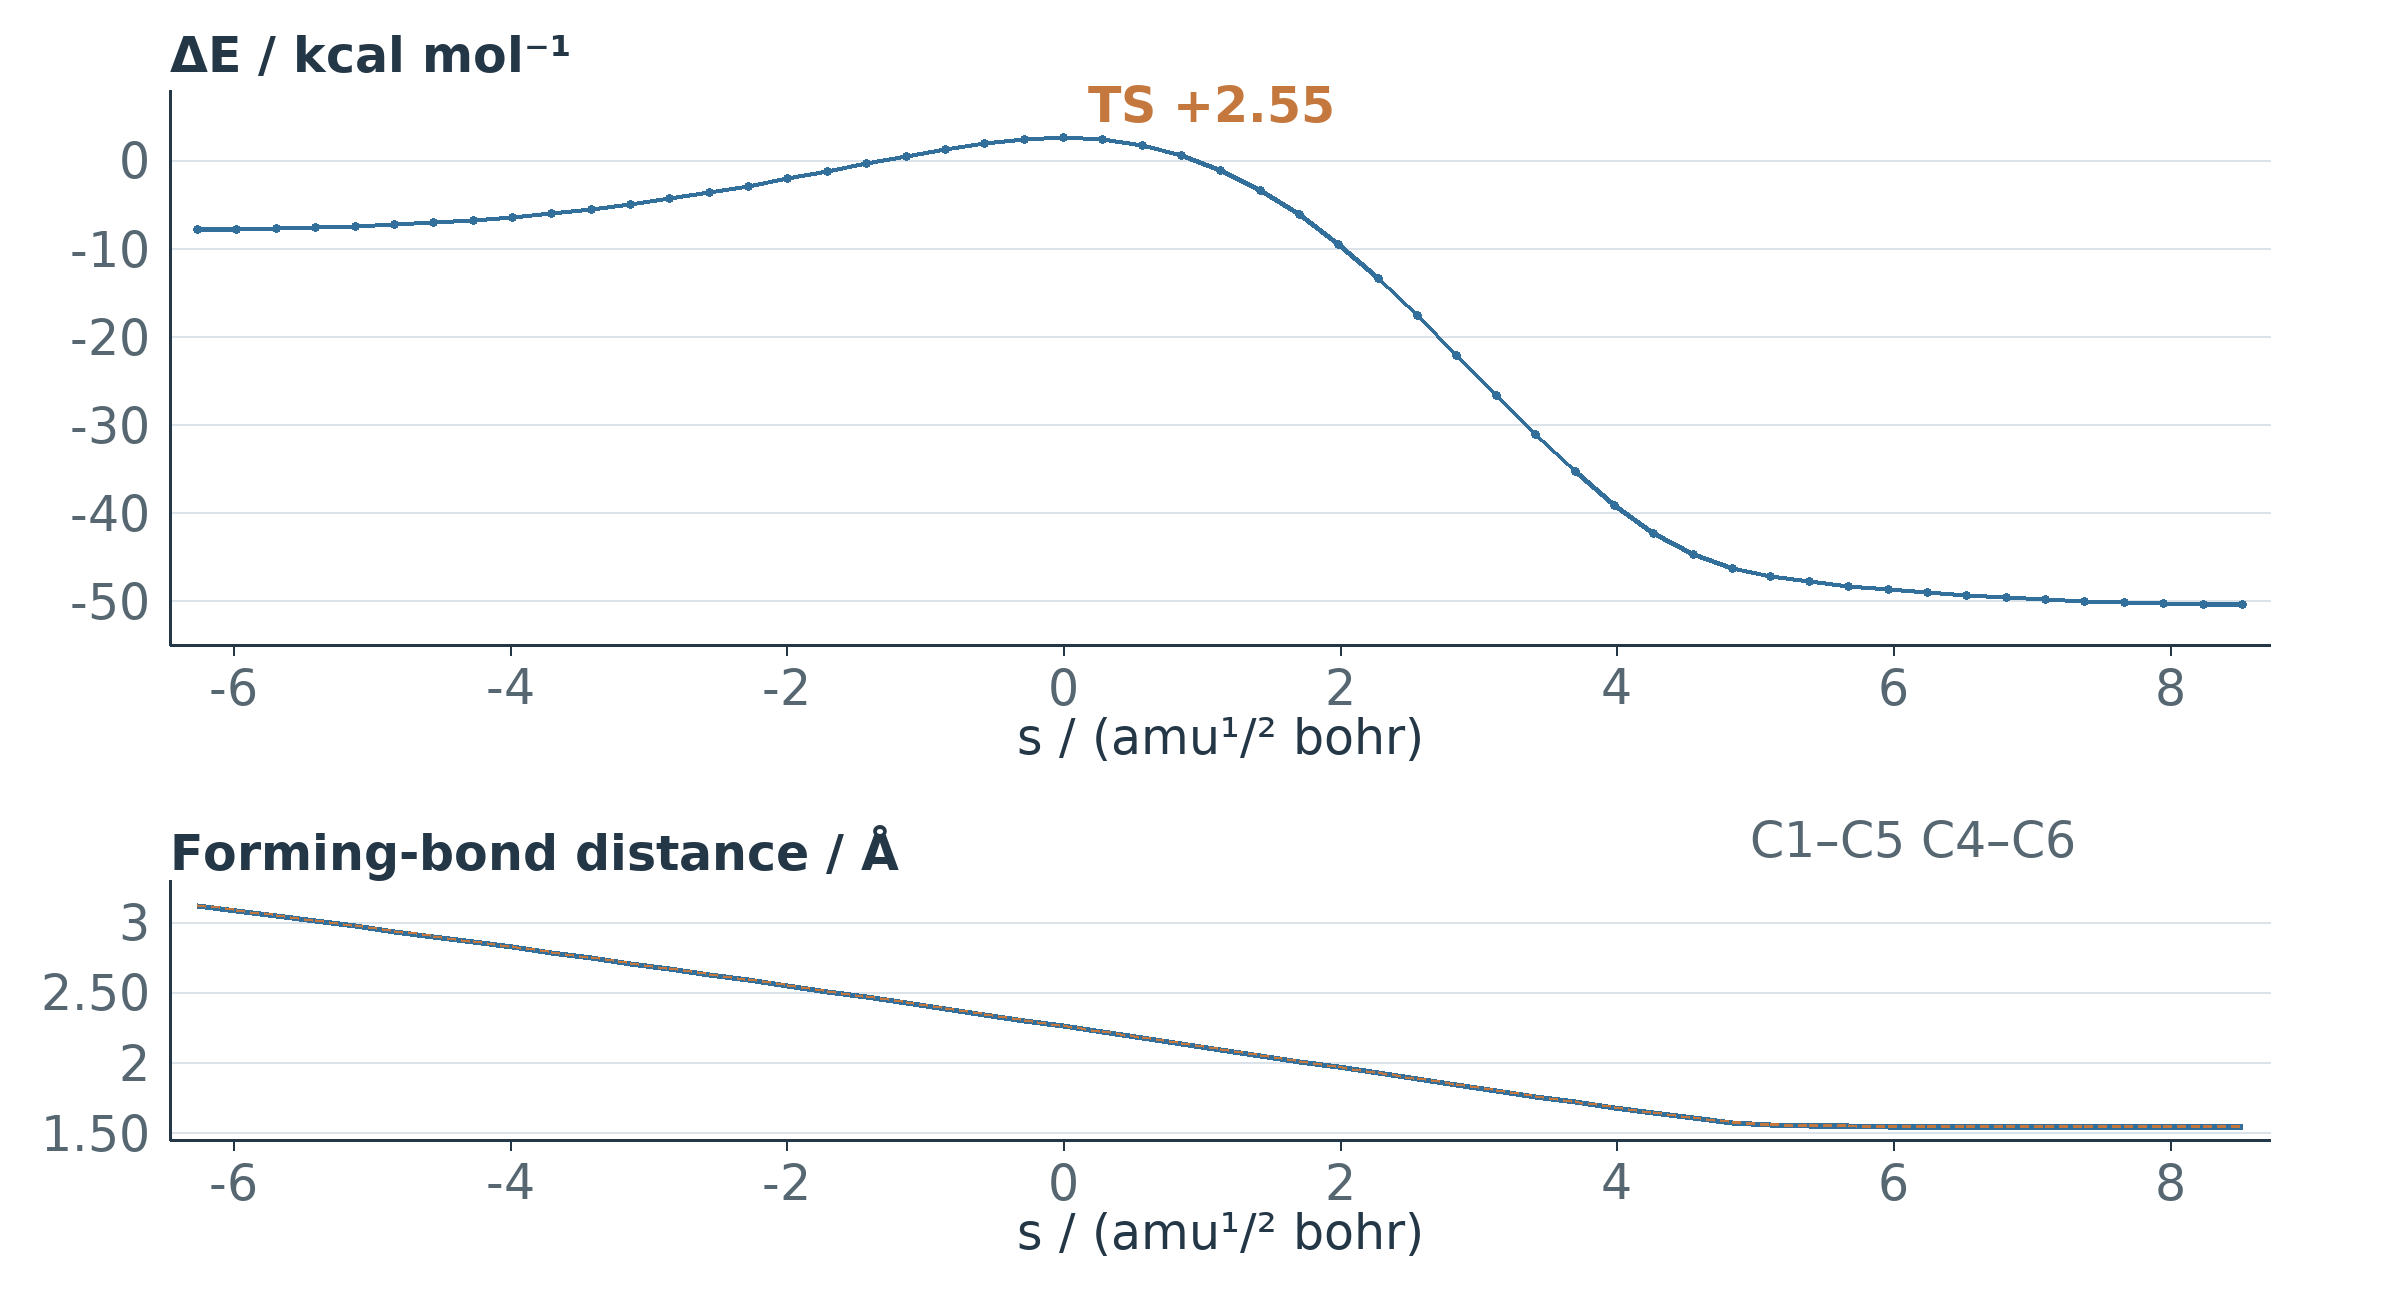
\includegraphics[width=\linewidth]{figures/maleic-gaussian-irc.png}
\caption{丁二烯与顺丁烯二酸酐反应的完整 Gaussian IRC，含反应物侧 22 点、产物侧 30 点及 TS。上图为相对于分离反应物的电子能，下图为两条形成键的距离；横轴为质量加权路径坐标，零点为过渡态。两端有限 IRC 点经独立优化和频率计算确认极小值。}
\label{fig:maleic-irc}
\end{figure}

以本次各程序的分离反应物能量之和为零点，Gaussian 与 ORCA 的电子能垒分别为 $2.55$、$2.55\ \kcalmol$。Gaussian 反应物复合物位于 $-7.84\ \kcalmol$，因此从复合物到过渡态的电子能高度为 $10.40\ \kcalmol$。复合物与分离反应物是不同参考态，二者给出的高度不应混称同一个双分子活化能。

\begin{table}[htbp]
\centering\small
\caption{顺丁烯二酸酐反应的相对电子能和 RRHO 自由能（$\kcalmol$）。各列以同程序分离反应物之和为零点；$G$ 已修正转动对称数。Gaussian 产物取 IRC 后优化极小值，ORCA 取独立优化的同一顺式构象。}
\label{tab:maleic-energy}
\begin{tabular}{lrrrr}
\toprule
物种 & Gaussian $\Delta E$ & ORCA $\Delta E$ & Gaussian $\Delta G$ & ORCA $\Delta G$\\
\midrule
分离反应物 & $0$ & $0$ & $0$ & $0$\\
反应物复合物 & $-7.84$ & --- & $2.26$ & ---\\
endo 过渡态 & $2.55$ & $2.55$ & $17.16$ & $17.23$\\
exo 过渡态 & $4.99$ & $4.99$ & $19.28$ & $19.42$\\
顺式产物 & $-50.42$ & $-50.42$ & $-32.21$ & $-32.15$\\
\bottomrule
\end{tabular}
\end{table}

转动对称数由元素及连接关系允许的原子置换与正旋转配准确定：丁二烯和顺丁烯二酸酐均为 2，复合物、过渡态及本次顺式产物构象均为 1。Gaussian 输出使用的对称数均为 1，因此双分子相对自由能统一减少 $2RT\ln 2=0.82\ \kcalmol$；ORCA 已采用相应的 2、2、1、1。由坐标、质量和全部实频重建的 RRHO 熵与两程序输出一致\cite{orca-thermo}。

在 $298.15\ \mathrm{K}$、$1\ \mathrm{atm}$ 下，活化自由能为 Gaussian $17.16$、ORCA $17.23\ \kcalmol$，产物反应自由能约为 $-32.2\ \kcalmol$。与乙烯反应的 $26.47\ \kcalmol$ 相比，顺丁烯二酸酐反应的 Gaussian 活化自由能低约 $9.31\ \kcalmol$。复合物电子能虽低于分离反应物，自由能仍高 $2.26\ \kcalmol$，反映双分子缔合的熵损失。复合物最低频率仅 $12.89\ \mathrm{cm^{-1}}$；这一能级对低频 RRHO 处理较敏感，而此处双分子活化自由能始终以分离反应物为参考。

\begin{figure}[htbp]
\centering
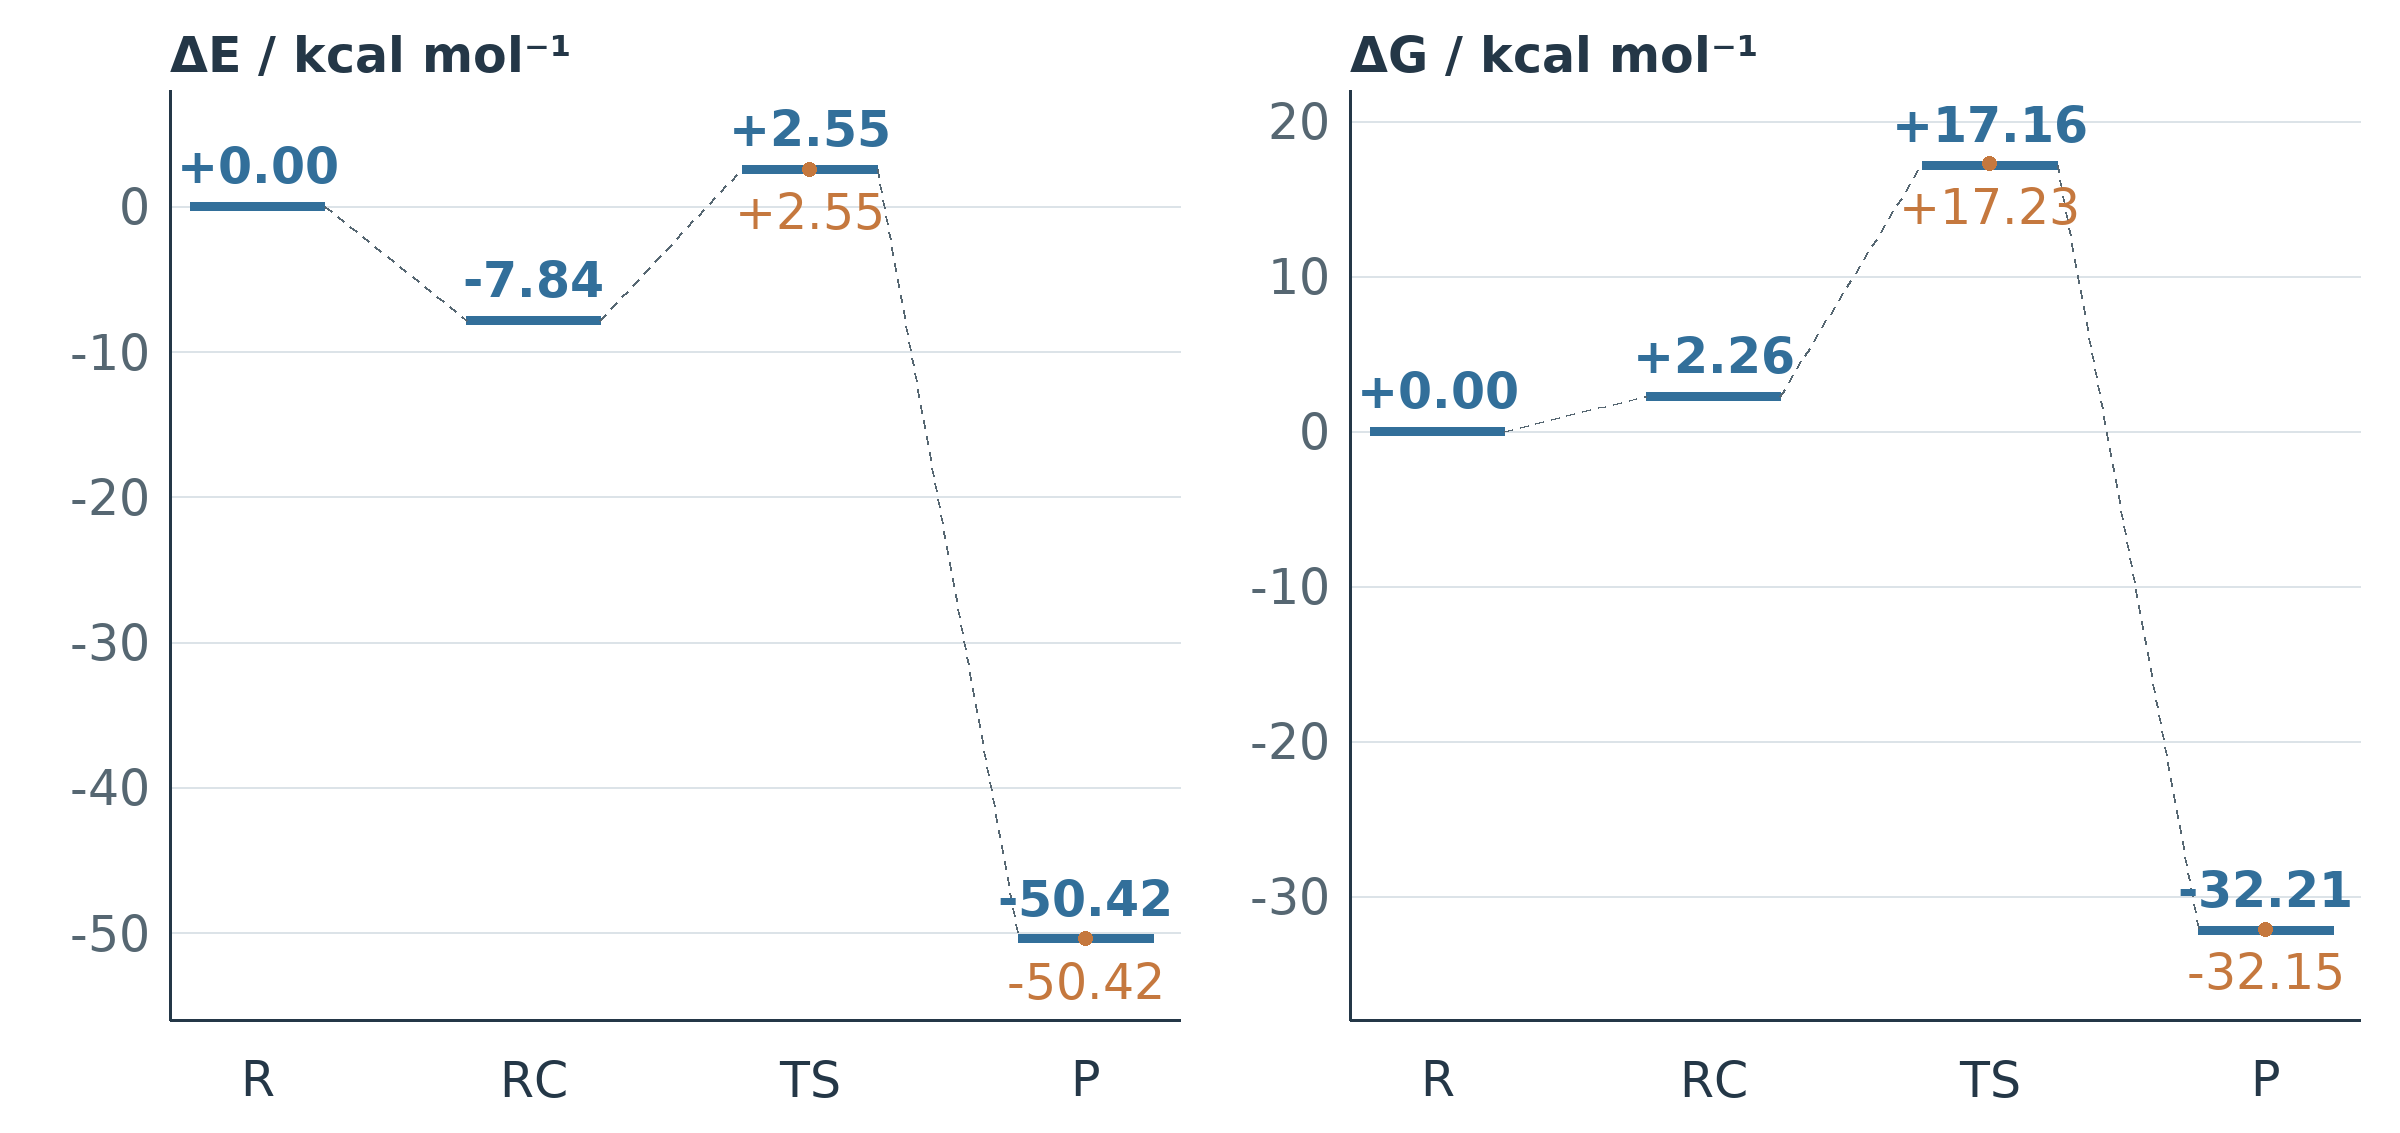
\includegraphics[width=\linewidth]{figures/maleic-energy-levels.png}
\caption{顺丁烯二酸酐反应的电子能及离散自由能阶梯。R、RC、TS、P 分别表示分离反应物、反应物复合物、过渡态和顺式产物。自由能为 $298.15\ \mathrm{K}$、$1\ \mathrm{atm}$ 下经转动对称数修正的 RRHO 结果。蓝线为 Gaussian 驻点，橙点为各自分离反应物基准下的 ORCA 结果。虚线仅指示能级次序，横向距离无路径长度含义；自由能图不是连续自由能反应路径。}
\label{fig:maleic-levels}
\end{figure}

由本次孤立反应物的 ORCA 波函数导出真实轨道等值面，得到丁二烯 HOMO 能量 $-6.52\ \mathrm{eV}$、顺丁烯二酸酐 LUMO 能量 $-3.35\ \mathrm{eV}$，轨道能隙为 $3.17\ \mathrm{eV}$。图~\ref{fig:maleic-frontier} 显示两者在反应碳端的相位分布。将孤立片段正旋转到过渡态的相对取向后，两组成键接触方向的相位积同号，可同时形成建设性重叠。该分析解释协同成键的轨道相容性，轨道能隙本身不等于活化能\cite{orca-plots}。

\begin{figure}[htbp]
\centering
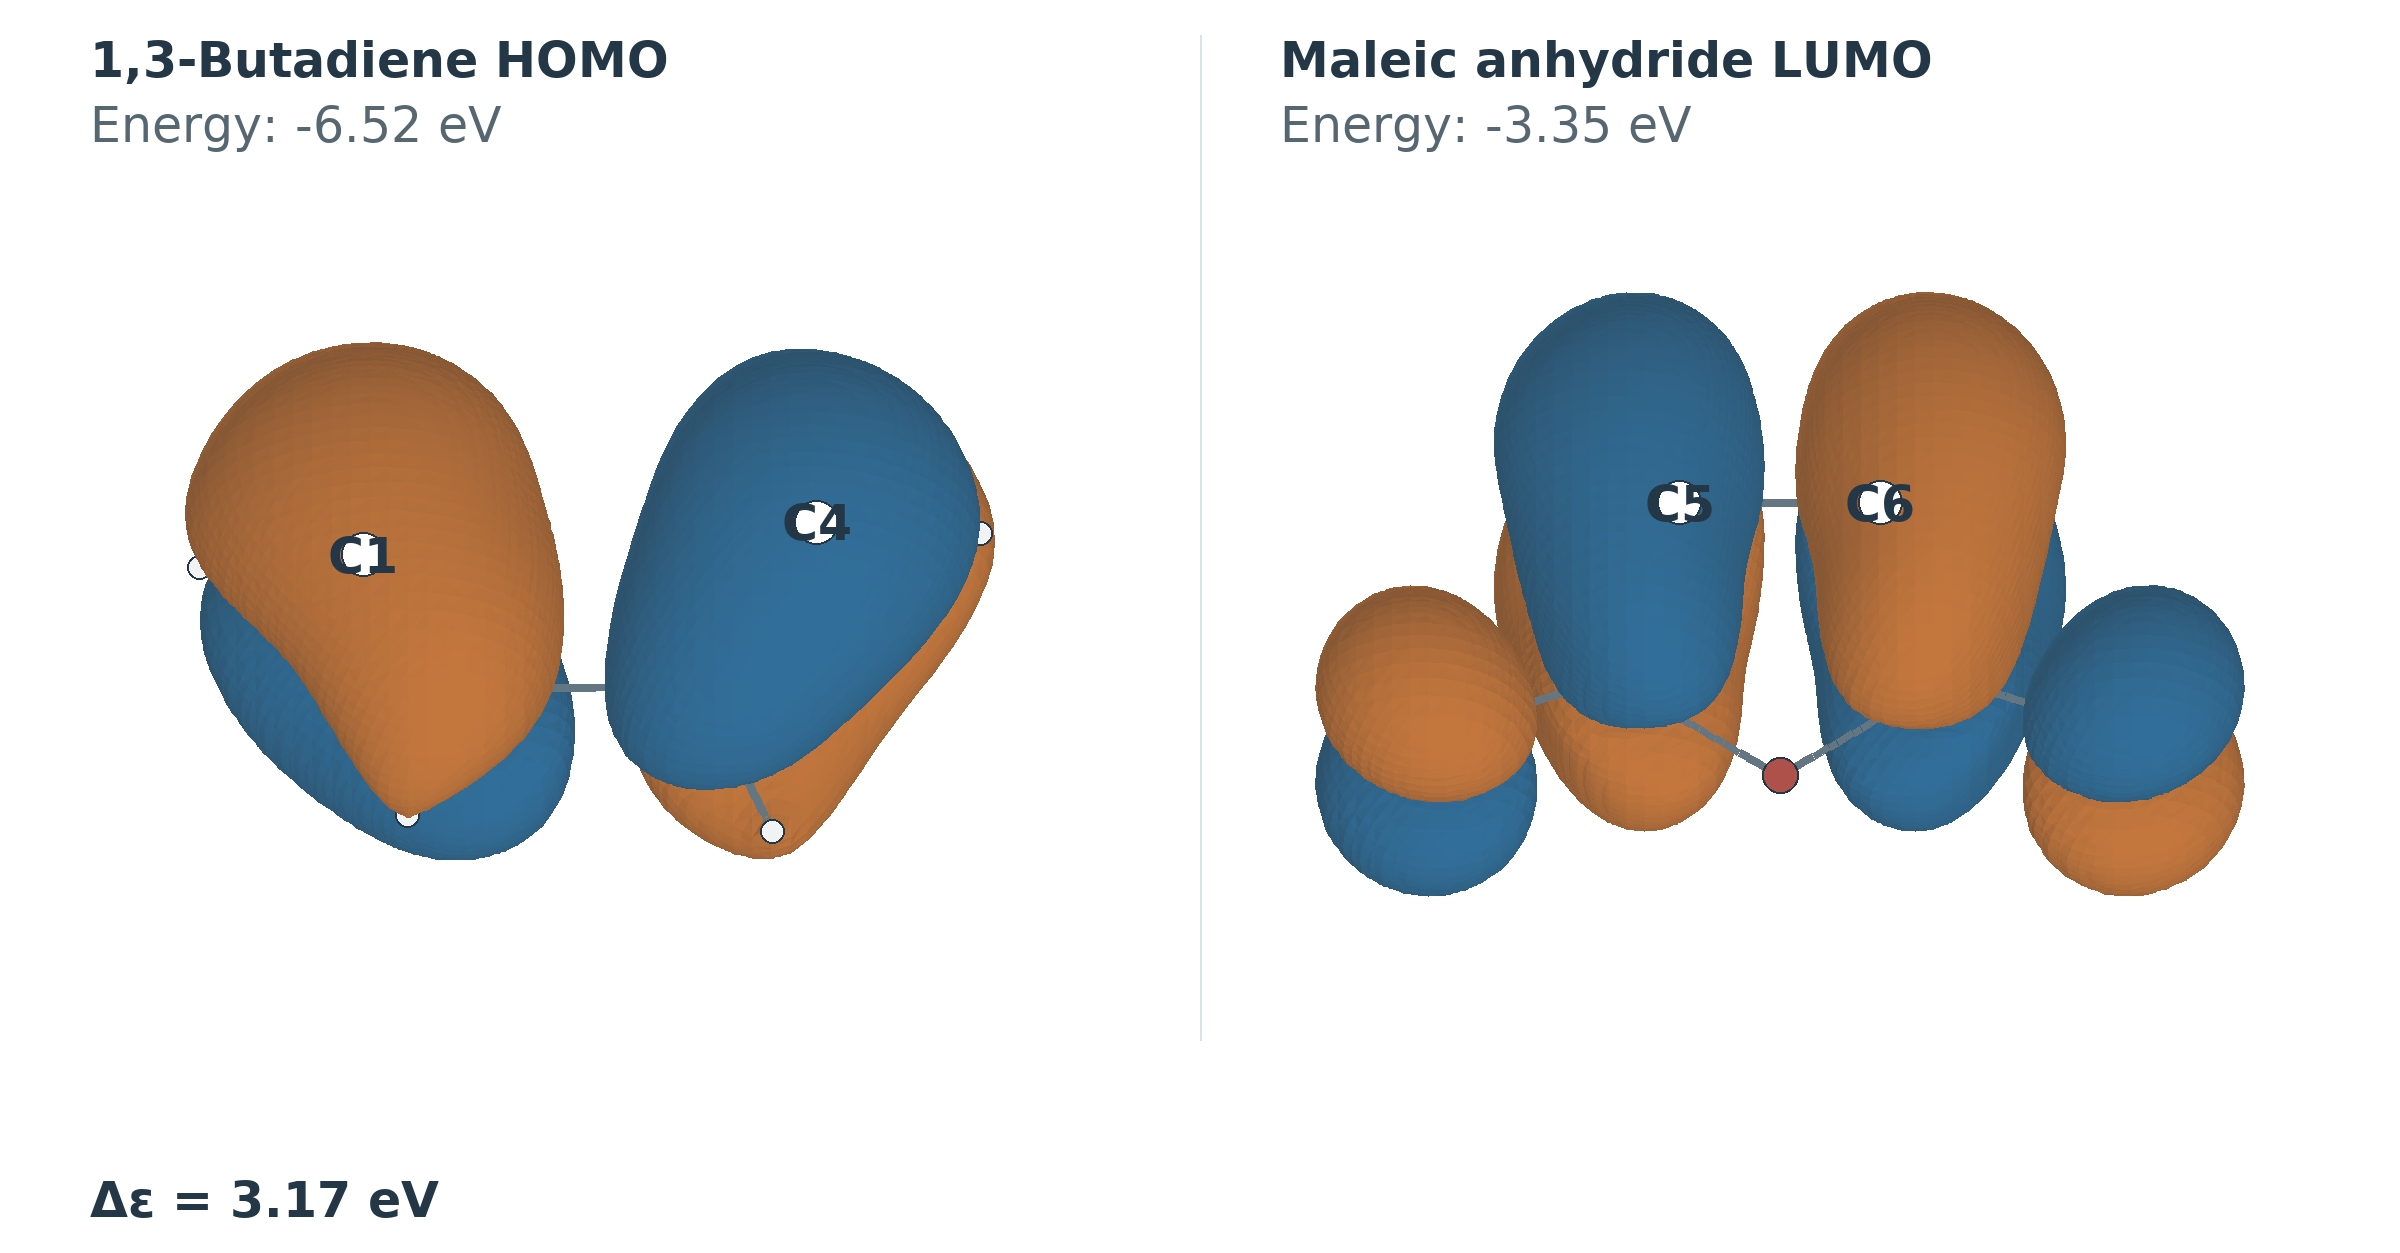
\includegraphics[width=\linewidth]{figures/maleic-frontier-phases.png}
\caption{本次独立优化反应物的丁二烯 HOMO 与顺丁烯二酸酐 LUMO。等值面为 $\pm0.030\ \mathrm{bohr^{-3/2}}$，蓝、橙两色表示相反相位，每个轨道的整体符号任意。所示为孤立片段轨道，图中标出参与成键的碳原子。}
\label{fig:maleic-frontier}
\end{figure}

exo 进攻的酸酐部分背离丁二烯内侧。Gaussian 与 ORCA 优化得到的 exo 过渡态分别具有唯一 $446.3i$、$445.6i\ \mathrm{cm^{-1}}$ 协同成键虚频，两条形成键均约为 $2.276\ \mathrm{\AA}$。两程序结构的正旋转配准 RMSD 为 $0.00011\ \mathrm{\AA}$，虚频模式重合度为 $0.99998$。

两种进攻过渡态的转动对称数均为 1。在相同分离反应物参照下，exo 相对 endo 的电子能高度为 Gaussian $2.44$、ORCA $2.43\ \kcalmol$；对应的活化自由能差为 $2.12$、$2.19\ \kcalmol$。两程序均支持 endo 进攻具有较低的活化自由能。

\begin{figure}[htbp]
\centering
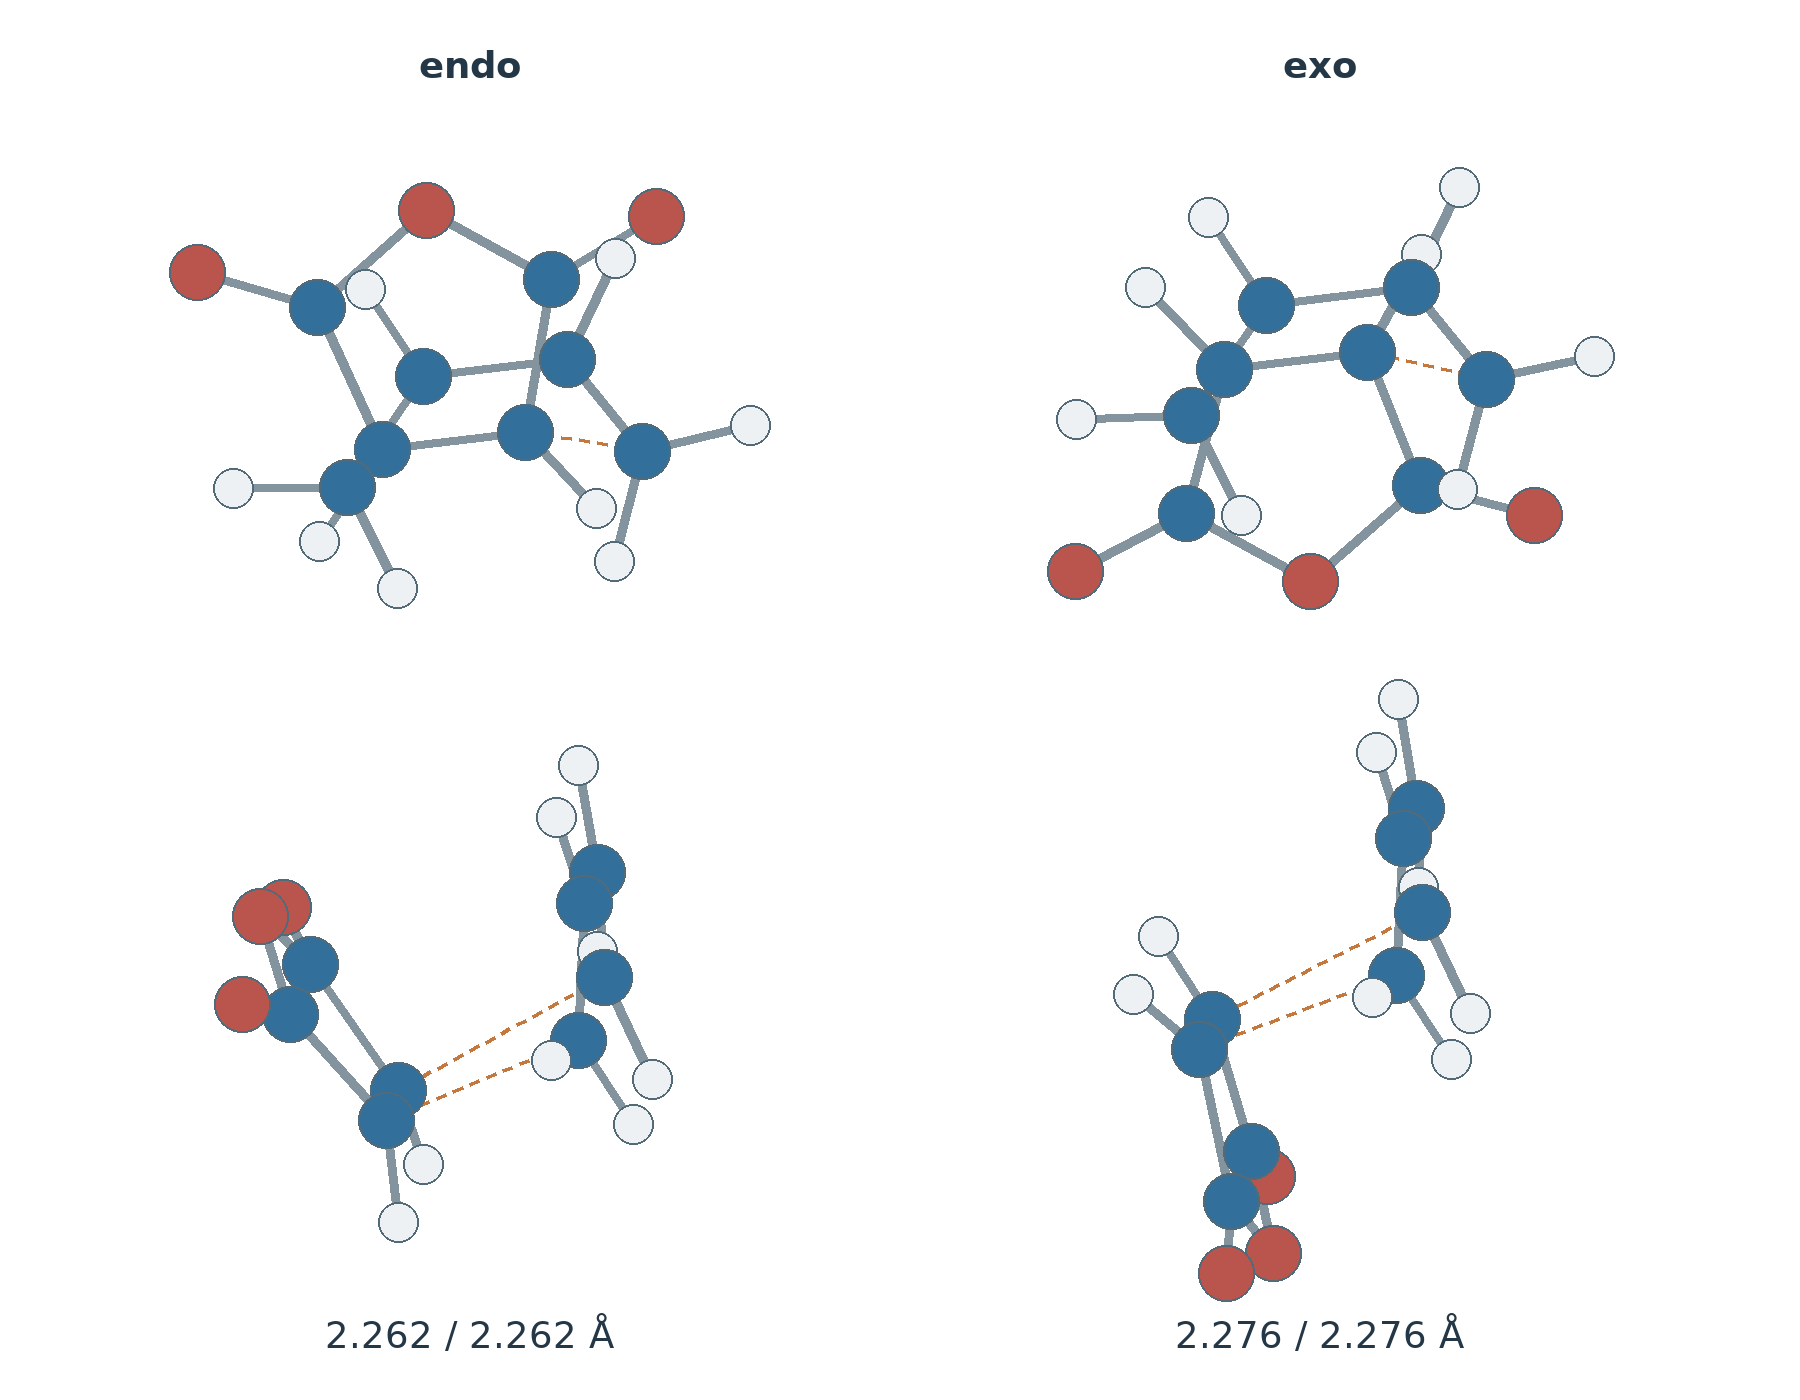
\includegraphics[width=\linewidth]{figures/maleic-endo-exo-ts.png}
\caption{Gaussian 优化的 endo 与 exo 过渡态正视（上）和侧视（下）对照。先按丁二烯 C1--C4 骨架作正旋转配准，再使用相同观察方向；蓝、红、浅灰分别表示 C、O、H。橙色虚线表示两条形成键，下方依次给出 C1--C5、C4--C6 距离。}
\label{fig:maleic-endo-exo-ts}
\end{figure}

\begin{figure}[htbp]
\centering
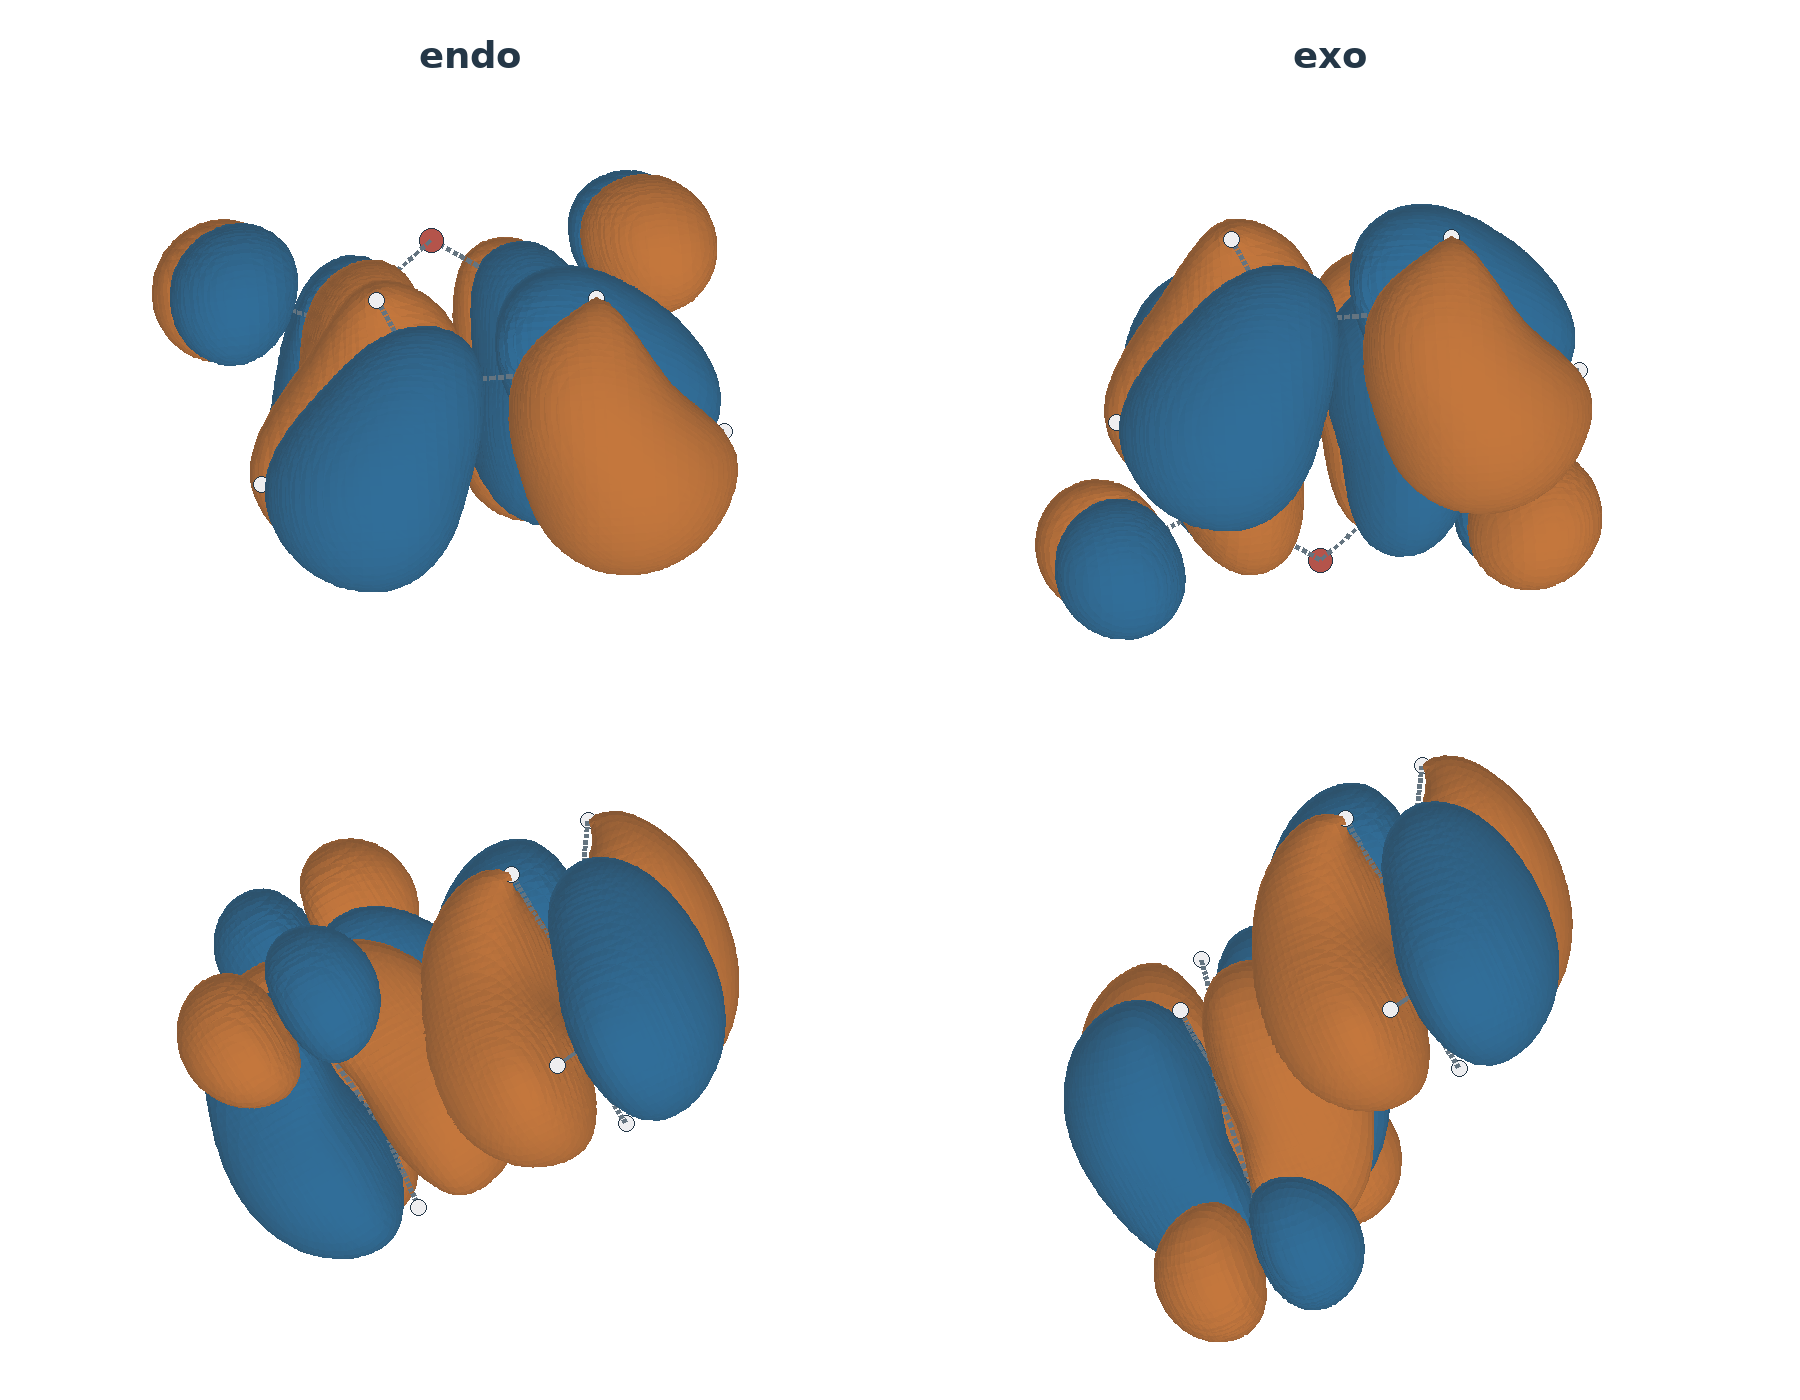
\includegraphics[width=\linewidth]{figures/maleic-orbital-endo-exo.png}
\caption{按 ORCA 的 endo、exo 过渡态朝向排列的丁二烯 HOMO 与酸酐 LUMO，上、下两排分别为统一视角的正视和侧视。等值面为 $\pm0.03\ \mathrm{bohr^{-3/2}}$，蓝、橙表示相反相位。孤立片段保持各自优化几何，仅作正旋转和平移；exo 图对 LUMO 作整体换号，使两幅图的相向叶瓣采用同一相位约定。两种朝向的两组成键接触均满足相位相容，但这一条件本身不能定量决定 endo/exo 的势垒差。}
\label{fig:maleic-orbital-comparison}
\end{figure}

配套动画分别展示两程序各自的 endo、exo 虚频运动，并提供同程序两朝向及同朝向两程序的并排对照。动画采用相同的显示振幅与播放相位，以比较协同成键方向；轨道动画则只改变观察角度。虚频位移不是实时动力学轨迹。

\begin{figure}[htbp]
\centering
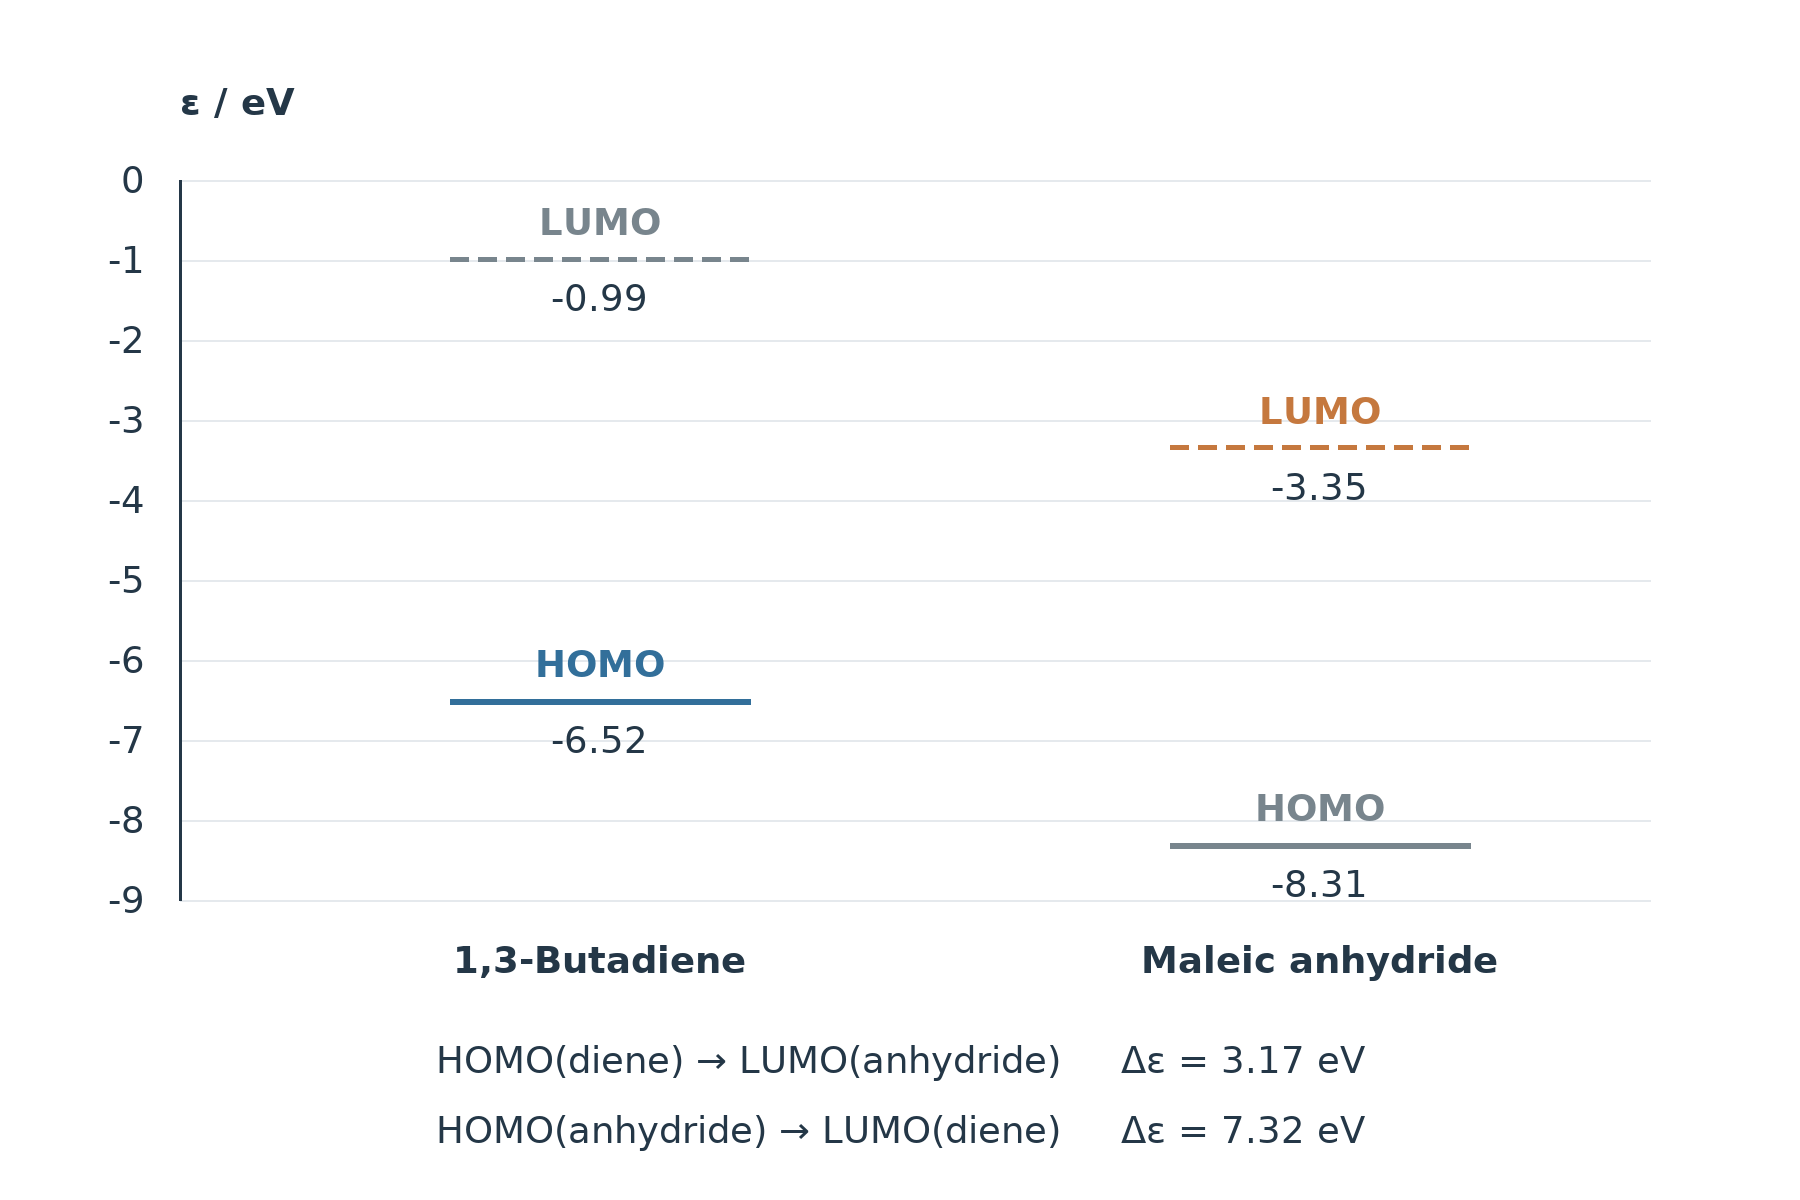
\includegraphics[width=\linewidth]{figures/maleic-frontier-levels.png}
\caption{丁二烯与顺丁烯二酸酐的孤立分子前线轨道能级，来自各自优化结构的 ORCA 波函数。实线为 HOMO，虚线为 LUMO；蓝色和橙色突出正常电子需求组合。丁二烯 HOMO--酸酐 LUMO 的能隙为 $3.17\ \mathrm{eV}$，反向组合为 $7.32\ \mathrm{eV}$。endo 与 exo 使用相同的孤立反应物能级，其差别在接近取向和相互作用；轨道能隙不等于活化能。}
\label{fig:maleic-frontier-levels}
\end{figure}

酸酐的低能 LUMO 使丁二烯 HOMO 向亲双烯体 LUMO 的供受体组合更有利。反向组合的能隙较大，因此本体系表现出正常电子需求的 Diels--Alder 特征。

\section{两种亲双烯体的统一对照}
两体系均以各自优化的近 s-cis 丁二烯与亲双烯体的分离分子之和为参照。表~\ref{tab:systems-energy} 将电子能和自由能分开比较；自由能统一为 $298.15\ \mathrm{K}$、$1\ \mathrm{atm}$ 下经转动对称数修正的 RRHO 结果。

\begin{table}[htbp]
\centering\small
\caption{两体系的能量对照，单位为 $\kcalmol$。上半表均为 Gaussian 结果；产物分别取 IRC 连接的环己烯 B 和酸酐顺式加成物，不以更稳定的环己烯 A 替代 B。exo 栏只列该朝向已确认的过渡态数据。下半表列 ORCA 的同程序参照结果。}
\label{tab:systems-energy}
\begin{tabular}{lrrr}
\toprule
比较量 & 乙烯 & 酸酐 endo & 酸酐 exo\\
\midrule
Gaussian $\Delta E^{\ddagger}$ & 12.95 & 2.55 & 4.99\\
Gaussian $\Delta G^{\ddagger}$ & 26.47 & 17.16 & 19.28\\
复合物 $\Delta E$ & $-2.79$ & $-7.84$ & ---\\
复合物 $\Delta G$ & 4.23 & 2.26 & ---\\
复合物至 TS 的电子能高度 & 15.74 & 10.40 & ---\\
产物 $\Delta E$ & $-45.81$ & $-50.42$ & ---\\
产物 $\Delta G$ & $-28.65$ & $-32.21$ & ---\\
\midrule
ORCA $\Delta E^{\ddagger}$ & --- & 2.55 & 4.99\\
ORCA $\Delta G^{\ddagger}$ & --- & 17.23 & 19.42\\
ORCA 复合物至峰顶电子能高度 & 15.74 & --- & ---\\
\bottomrule
\end{tabular}
\end{table}

在相同 Gaussian 模型和参照约定下，酸酐 endo、exo 的活化自由能分别比乙烯低 $9.31$、$7.19\ \kcalmol$；酸酐 endo 比 exo 低 $2.12\ \kcalmol$。两体系均放能且反应自由能为负，酸酐 endo 产物的反应自由能比环己烯 B 更负 $3.56\ \kcalmol$。乙烯的 ORCA 路径高度以弱复合物为参照，故单独列出，不与分离反应物基准的活化能混合。

\begin{table}[htbp]
\centering\small
\caption{两体系过渡态的结构和唯一成键虚频。两距离分别为 C1--C5、C4--C6，单位为 $\mathrm{\AA}$；虚频单位为 $\mathrm{cm^{-1}}$。乙烯 ORCA 一行取经独立频率核验的 CI-NEB 峰顶，其余为无约束优化过渡态。}
\label{tab:systems-ts}
\begin{tabular}{llrrr}
\toprule
亲双烯体／朝向 & 程序 & $r_1$ & $r_2$ & 虚频\\
\midrule
乙烯 & Gaussian & 2.271 & 2.271 & $517.2i$\\
乙烯 & ORCA & 2.271 & 2.271 & $516.1i$\\
酸酐 endo & Gaussian & 2.262 & 2.262 & $443.0i$\\
酸酐 endo & ORCA & 2.262 & 2.262 & $443.0i$\\
酸酐 exo & Gaussian & 2.276 & 2.276 & $446.3i$\\
酸酐 exo & ORCA & 2.276 & 2.276 & $445.6i$\\
\bottomrule
\end{tabular}
\end{table}

两体系的两条形成键均近乎等长，虚频均对应协同成键。酸酐 endo 的形成键比乙烯略短，exo 则略长；虚频绝对值的大小描述鞍点附近反应坐标方向的曲率，不直接代表势垒高低。

\begin{table}[htbp]
\centering\small
\caption{两体系孤立反应物的前线轨道对照，单位为 eV。乙烯体系取 Gaussian 波函数，酸酐体系取 ORCA 波函数，均为本报告的 B3LYP-D3(BJ)/def2-SVP 模型；两程序的积分网格不同。酸酐 endo/exo 共用同一组孤立分子能级。正常、反向能隙分别为亲双烯体 LUMO 减丁二烯 HOMO、丁二烯 LUMO 减亲双烯体 HOMO。}
\label{tab:systems-orbitals}
\begin{tabular}{lrr}
\toprule
比较量 & 丁二烯＋乙烯 & 丁二烯＋酸酐\\
\midrule
丁二烯 HOMO & $-6.52$ & $-6.52$\\
丁二烯 LUMO & $-0.99$ & $-0.99$\\
亲双烯体 HOMO & $-7.51$ & $-8.31$\\
亲双烯体 LUMO & $0.15$ & $-3.35$\\
正常电子需求能隙 & 6.67 & 3.17\\
反向电子需求能隙 & 6.52 & 7.32\\
\bottomrule
\end{tabular}
\end{table}

相较乙烯，酸酐显著降低了亲双烯体 LUMO，使正常电子需求能隙缩小约 $3.49\ \mathrm{eV}$。这一趋势与酸酐较低的环加成势垒一致，但势垒还取决于片段形变及相互作用，不能由轨道能隙直接换算。endo/exo 的孤立轨道能级相同，其选择性需结合不同接近取向下的过渡态自由能判断。

\section{思考与讨论}
\subsection{为什么一阶过渡态恰有一个虚频？}
在驻点附近作二阶展开：
\begin{equation}
E\simeq E_0+\frac12\sum_i\lambda_i Q_i^2.
\end{equation}
一阶鞍点沿一个方向为极大值、沿其余振动方向为极小值，因此恰有一个 $\lambda_i<0$，对应虚频。没有虚频通常对应极小值；多个虚频对应更高阶鞍点。数值上还须排除未收敛几何引起的伪虚频。本次 $517.2i\ \mathrm{cm^{-1}}$ 模式对应两条 C--C 键的协同变化，且 IRC 确认其连接关系，因而能够将该鞍点归属为所研究环加成通道的过渡态\cite{transition-state}。

\subsection{过渡态理论的基本假设是什么？}
常规过渡态理论将反应速率视为体系穿过反应物与产物之间分界面的通量。其主要假设为：反应物区能够建立热平衡；反应物与除去反应坐标自由度的活化复合体保持准平衡；沿反应坐标的运动可与其余自由度近似分离；向产物方向穿过分界面的轨迹不再返回\cite{tst}。

对于单分子步骤，Eyring 形式为
\begin{equation}
k_1=\kappa\frac{k_{\rm B}T}{h}
\exp\!\left(-\frac{\Delta G^{\ddagger,\circ}}{RT}\right).
\end{equation}
本实验是双分子反应，若以浓度定义二级速率常数，则需匹配标准态：
\begin{equation}
k_2=\kappa\frac{k_{\rm B}T}{h}\frac{1}{c^\circ}
\exp\!\left(-\frac{\Delta G^{\ddagger,\circ}}{RT}\right),
\qquad c^\circ=\frac{p^\circ}{RT}.
\end{equation}
本报告 $p^\circ=1\ \mathrm{atm}$。常规无再穿越近似取 $\kappa=1$；反应坐标对应的虚频不作为稳定谐振动计入配分函数。

\subsection{过渡态理论有哪些不适用或需要修正的情形？}
显著的分界面再穿越会使无再穿越近似高估反应通量；轻原子转移及低温反应中的隧穿使经典越垒描述不足；未达到热平衡的短寿命中间体或强非统计动力学不满足准平衡假设。涉及电子态切换的反应还需要非绝热动力学；无明显势能鞍点的缔合、扩散控制反应也不能仅用某个鞍点的谐振子自由能描述。因而，IRC 确定的是势能面上的连接通道，不等同于真实时间轨迹或完整速率模型。

\section{结论}
在 B3LYP-D3(BJ)/def2-SVP 水平上，1,3-丁二烯与乙烯环加成过渡态具有唯一的 $517.2i\ \mathrm{cm^{-1}}$ 虚频，两条形成键约为 $2.271\ \mathrm{\AA}$。双向 IRC 与端点频率计算确认该通道连接丁二烯--乙烯弱结合复合物和环己烯 B，沿路径呈现近同步的双端成键。丁二烯 HOMO 与乙烯 LUMO 在两端可同时满足同相重叠，为协同成键提供轨道解释。

以各自程序的弱结合复合物为参照，普通 NEB、CI-NEB 与原 Gaussian TS 的电子势垒分别为 $15.74$、$15.74$、$15.74\ \kcalmol$。CI-NEB 峰顶具有唯一的 $516.1i\ \mathrm{cm^{-1}}$ 成键虚频，其几何与模式均与原 TS 高度一致。NEB/CI-NEB 与 IRC 在势垒顶和整体成键趋势上相符，主要差别位于反应物侧的路径形状及有限 IRC 末点。

以所优化的近 s-cis 扭曲丁二烯与乙烯为参考，$298.15\ \mathrm{K}$、$1\ \mathrm{atm}$ 下经转动对称数修正的 RRHO 活化自由能为 $26.47\ \kcalmol$，生成 B 的反应自由能为 $-28.65\ \kcalmol$。构象 A 更稳定，其相对自由能为 $-32.94\ \kcalmol$。构象 CI-NEB 和鞍点精修给出相对 A、B 的电子能高度分别为 $5.59$、$0.027\ \kcalmol$，说明 B 位于环扭转势能面上很浅的局部势阱中。

顺丁烯二酸酐反应的 Gaussian 与 ORCA 电子能垒均约为 $2.55\ \kcalmol$，活化自由能分别为 $17.16$、$17.23\ \kcalmol$。唯一的约 $443i\ \mathrm{cm^{-1}}$ 成键虚频及 Gaussian 双向 IRC 确认了反应物复合物到顺式加成产物的通道；相较乙烯，顺丁烯二酸酐在同一模型和单构象参照下具有更低的环加成势垒。

\begin{thebibliography}{99}
\bibitem{course} 刘迎春. 环加成反应的机理研究：量子化学实验课件. 浙江大学化学系，2026年10月，pp. 2--5, 8--26.
\bibitem{thermo} Ochterski, J. W. \textit{Thermochemistry in Gaussian}. Gaussian, Inc., 2000; updated 2022. \url{https://gaussian.com/wp-content/uploads/dl/thermo.pdf}.
\bibitem{transition-state} IUPAC. Transition state. \textit{Compendium of Chemical Terminology (the Gold Book)}. \url{https://doi.org/10.1351/goldbook.T06468}.
\bibitem{tst} IUPAC. Transition state theory. \textit{Compendium of Chemical Terminology (the Gold Book)}. \url{https://doi.org/10.1351/goldbook.T06470}.
\bibitem{orca-dft} FACCTs. \textit{ORCA 6.1 Manual}, Density Functional Theory. \url{https://www.faccts.de/docs/orca/6.1/manual/contents/modelchemistries/DensityFunctionalTheory.html}.
\bibitem{orca-freq} FACCTs. \textit{ORCA 6.1 Manual}, Vibrational Frequencies. \url{https://www.faccts.de/docs/orca/6.1/manual/contents/structurereactivity/frequencies.html}.
\bibitem{ase-neb} ASE developers. \textit{Nudged elastic band}, Climbing image and analysis of output. \url{https://docs.ase-lib.org/ase/neb.html}.
\bibitem{orca-irc} FACCTs. \textit{ORCA 6.1 Manual}, Intrinsic Reaction Coordinate. \url{https://www.faccts.de/docs/orca/6.1/manual/contents/structurereactivity/irc.html}.
\bibitem{orca-thermo} FACCTs. \textit{ORCA 6.1 Manual}, Thermochemistry. \url{https://www.faccts.de/docs/orca/6.1/manual/contents/structurereactivity/thermochemistry.html}.
\bibitem{orca-plots} FACCTs. \textit{ORCA 6.1 Manual}, Orbital and Density Plots. \url{https://www.faccts.de/docs/orca/6.1/manual/contents/utilitiesvisualization/plots.html}.
\end{thebibliography}
\section*{数据与代码}
本实验的计算结果、图表、后处理脚本及报告源文件公开于：

\noindent\url{https://github.com/populuscathayana/Quantum3}
\end{document}
